\chapter{Agent--Based Data Augmentation for Fitting Stochastic Epidemic Models to Prevalence Data}
\label{chap:bda_for_fitting_sems_to_prevalence_data}

\section{Overview}
\label{sec:bda_overview}

Stochastic epidemic models (SEMs) are classic tools for modeling the spread of infectious diseases. A SEM represents the time evolution of an epidemic in terms of the disease histories of individuals as they transition through disease states. Incorporating stochasticity into epidemic models is important when the disease prevalence is low or when the population size is small. In both cases, the stochastic variability in the evolution of an epidemic greatly influences the probability of an outbreak, its severity, and the conclusions we draw about its dynamics \cite{allen2008introduction,keeling2008}. Moreover, many questions --- e.g., what is the final size distribution? What is the probability that a disease has been eradicated? --- cannot be answered using deterministic methods \cite{britton2010}.

The task of fitting a SEM is typically complicated by the limited extent of epidemiological data, which are recorded at discrete observation times, commonly describe just one aspect of the disease process, e.g., infections, and usually capture only a fraction of cases. Complete subject--level data, which would consist of the exact times at which individuals transition through disease states, are often unavailable \cite{oneill2010}. Fitting SEMs in the absence of complete subject--level data presents a complicated latent variable problem since it is usually impossible to analytically integrate over the missing data \cite{oneill2002}. This makes the observed data likelihood for a SEM intractable.

Agent--based data augmentation (DA) methods for fitting SEMs, first presented in \cite{gibson1998} and \cite{oneill1999}, target the joint posterior distribution of the missing data and model parameters to obtain a tractable complete data likelihood. That the augmentation is agent--based refers to the introduction of subject--level disease histories, rather than population--level epidemic paths, as latent variables in the model. An advantage of the agent--based approach is that household structure and subject--level covariates may be incorporated into the model \cite{auranen2000,hohle2002,cauchemez2004bayesian, neal2004statistical,oneill2009}. Development of DA methods for SEMs is of continuing interest, and recent works by \cite{pooley2015}, \cite{QinShe15}, and \cite{shestopaloff2016sampling} have presented methods that could possibly be applied to epidemic count data. However, their algorithms forgo the flexibility of agent--based DA and, in the case of the latter two papers, have not been applied to SEMs.

We present an agent--based DA Markov chain Monte Carlo (MCMC) framework for fitting SEMs to time series count data of disease prevalence. We obtain a tractable complete data likelihood by augmenting the data with subject--level disease histories. Our MCMC targets the joint posterior distribution of the latent epidemic process and the model parameters as we alternate between updating subject--level paths and model parameters. We propose each new subject--path, conditionally on the data, using a time--inhomogeneous continuous--time Markov chain (CTMC) with rates determined by the disease histories of the other individuals. These data--driven path proposals result in highly efficient perturbations to the latent epidemic path, and enable us to analyze epidemic count data in the absence of any subject--level information. In contrast, traditional agent--based DA MCMC algorithms rely on data--agnostic trans--dimensional proposals and suffer from convergence issues as the fraction of missing information becomes large \cite{roberts2001, mckinley2014simulation, pooley2015}. The \textit{de facto} need for some subject--level data has precluded the use of classical DA machinery in many settings. Thus, our MCMC algorithm enables exact Bayesian inference for SEMs fit to datasets that would have been impossible to study with existing agent--based DA methods. Our algorithm is not specific to any particular SEM dynamics or measurement process, and may be applied, with minimal modifications, to a broad class of SEMs. 

\section{The data augmentation algorithm for an SIR model}
\label{sec:bda_sir_model}

For concreteness and clarity of exposition, we present our Bayesian DA algorithm (BDA) in the context of fitting a stochastic Susceptible--Infected--Recovered (SIR) model to binomially distributed prevalence counts. We also use our algorithm to fit Susceptible--Exposed--Infected--Recovered (SEIR) and Susceptible--Infected--Recovered--Susceptible (SIRS) models in Sections \ref{subsec:bda_sir_seir_sirs_sim}, \ref{subsec:bda_misspec_sim}, and \ref{sec:bda_bbs}, and outline the minimal adaptations required for these models in Sections \ref{subsec:bda_seir_model} and \ref{subsec:bda_sirs_model}.

The SIR model describes the time evolution of an epidemic in terms of the disease histories of individuals as they transition through three states --- susceptible (S), infected/infectious (I), and recovered (R). Under simple SIR dynamics, each individual becomes infectious immediately upon becoming infected, and acquires lifelong immunity upon recovery. For simplicity, we assume that the population is closed and mixes homogeneously, and that there is no external force of infection. Therefore, the epidemic ceases once the pool of infectious individuals is depleted.

\subsection{Measurement process and data}
\label{subsec:bda_meas_proc}
Our data, $\bY = \lbrace Y_{1}, \dots, Y_L \rbrace$, are disease prevalence counts recorded at times $t_1,\dots,t_L \in [t_1,t_L]$. It should not beggar belief that the data could be subject to measurement error, for example underreporting in settings where asymptomatic individuals escape detection. Let $ S_\tau $, $ I_\tau $, and $ R_\tau $ denote the total susceptible, infected, and recovered people at time $ \tau $. We model the observed prevalence as a binomial sample, with constant mean case detection probability $ \rho $. Thus,
\begin{equation}\label{eqn:bda_emit_dist}
Y_\ell | I_{t_\ell},\rho \sim \mathrm{Binomial}\left (I_{t_\ell}, \rho\right ).\end{equation}

\subsection{Latent epidemic process}
\label{subsec:bda_pop_proc}
The data are sampled from a latent epidemic process, $ \bX = \lbrace \bX_1,\dots,\bX_N\rbrace $, that evolves continuously in time  as individuals become infected and recover. The state space of this process is $ \mcS = \lbrace S,I,R\rbrace^N $, the Cartesian product of $ N $ state labels taking values in $ \lbrace S,I,R\rbrace $. The state space of a single subject, $ \bX_j $, is $\mcS_j = \lbrace S, I, R\rbrace $, and a realized subject--path is of the form 
\begin{equation} \bx_j(\tau) = \left \lbrace \begin{array}{ll}
S\ ,& \tau < \tau^{(j)}_{\mathrm{I}},\\
I\ ,& \tau^{(j)}_{\mathrm{I}} \leq \tau < \tau^{(j)}_{\mathrm{R}},\\
R\ ,& \tau^{(j)}_{\mathrm{R}} \leq \tau,
\end{array} \right . \end{equation} 
where $ \tau^{(j)}_{\mathrm{I}} $ and $ \tau^{(j)}_{\mathrm{R}} $ are the infection and recovery times for subject $ j $ (though subject $ j $ may also never become infected or recover, or may become infected or recover outside of the observation period $ [t_1,t_L] $). We write the configuration of $ \bX $ at time $ \tau $ as $ \bX(\tau) = \left (\bX_1(\tau),\dots,\bX_N(\tau)\right ) $, and adopt the convention that $ \bX(\tau) $ and derived quantities, e.g., $ I_\tau $, depend on the configuration just before $ \tau $. We  use $ \tau^+ $ for quantities evaluated just after a particular time. The waiting times between transition events are taken to be exponentially distributed, and we denote by $ \beta $ and $ \mu $ the per--contact infectivity and recovery rates. Thus, the latent epidemic process evolves according to a time--homogeneous CTMC, with transition rate from configuration $ \bX $ to $ \bX^\prime $ given by
\begin{equation}
\lambda_{\bX,\bX^\prime} = \left \lbrace \begin{array}{rl}
\beta I,\ &\text{if } \bX\ \text{and } \bX^\prime\ \text{differ only in subject }j \text{, with }\bX_j=S\text{, and }\bX_j^\prime=I,\\
\mu,\ &\text{if } \bX\ \text{and } \bX^\prime\ \text{differ only in subject }j \text{, with }\bX_j=I\text{, and }\bX_j^\prime=R,\\
0,\ & \text{for all other configurations }\bX\ \text{and }\bX^\prime.
\end{array}\right.
\end{equation}
At the first observation time, we let $ \bX(t_1)|\bp_{t_1} \sim \mathrm{Categorical}\left (\lbrace S,I,R\rbrace, \bp_{t_1}\right ) $, where $ \bp_{t_1}=\left(p_{S}, p_{I},p_{R}\right) $ are the probabilities that an individual is susceptible, infected, or recovered. Let $ \btau = \lbrace\tau_0,\dots,\tau_{K+1}\rbrace $, where $ t_1 \equiv \tau_0 $ and $ t_L \equiv \tau_{K+1} $, be the (ordered) set of $ K $ infection and recovery times of all individuals along with the endpoints of the observation period $ [t_1,t_L] $. Let $ \ind{\tau_k \corresponds I} $ and $ \ind{\tau_k \corresponds R} $ indicate whether $ \tau_k $ is an infection or recovery time, and let $ \btheta = (\beta, \mu, \rho, \bp_{t_1}) $ denote the vector of unknown parameters. The complete data likelihood is 
\begin{align} 
\label{eqn:bda_comp_data_likelihood}
L(\bX, \bY | \btheta) &= \Pr(\bY|\bX, \rho)\times \Pr(\bX(t_1)|\bp_{t_1}) \times \pi(\bX |\bX(t_1),\beta, \mu) \nonumber \\
&=  \left [ \prod_{l = 1}^{L}\binom{I_{t_\ell}}{Y_\ell}  \rho^{Y_\ell}(1-\rho)^{I_{t_\ell} - Y_\ell}\right ] \times \left [p_{S}^{S_{t_1}} p_{I}^{I_{t_1}}p_{R}^{R_{t_1}}\right ]  \nonumber\\
&\hspace{0.2in} \times \prod_{k = 1}^{K}\left \lbrace \left [\beta I_{\tau_k}\times\ind{\tau_k \corresponds I} + \mu\times\ind{\tau_k \corresponds R}\right ] \exp{\left [-\left (\tau_k - \tau_{k-1}\right )\left (\beta I_{\tau_k} S_{\tau_k} + \mu I_{\tau_k}\right )\right ]}\right \rbrace \nonumber \\
& \hspace{0.2in} \times \exp \left [-\left (t_L - \tau_K\right )\left (\beta I_{\tau_K^+}S_{\tau_K^+} + \mu I_{\tau_K^+}\right )\right ]. 
\end{align}
We briefly reconcile what might seem like a discrepancy between the SIR model presented above and the lumped construction of the SIR model (see \cite{andersson2000stochastic}), which is common for a number of computational and analytical reasons. Our model describes the time evolution of the subject--level collection of disease histories, and thus evolves on the state space of individual disease labels. The lumped SIR model describes the time evolution of the vector of compartment counts, the state space of which is defined as the partition of the original state space obtained by aggregating the individuals in each of the model compartments. The lumped construction would have been appropriate had we chosen to augment the data with the compartment counts (for example, as in \cite{pooley2015}). Nonetheless, inference based on the full subject--level model will exactly match inference based on the lumped model. We discuss this further in Section \ref{sec:lumpability}.

\begin{figure}
	\centering
	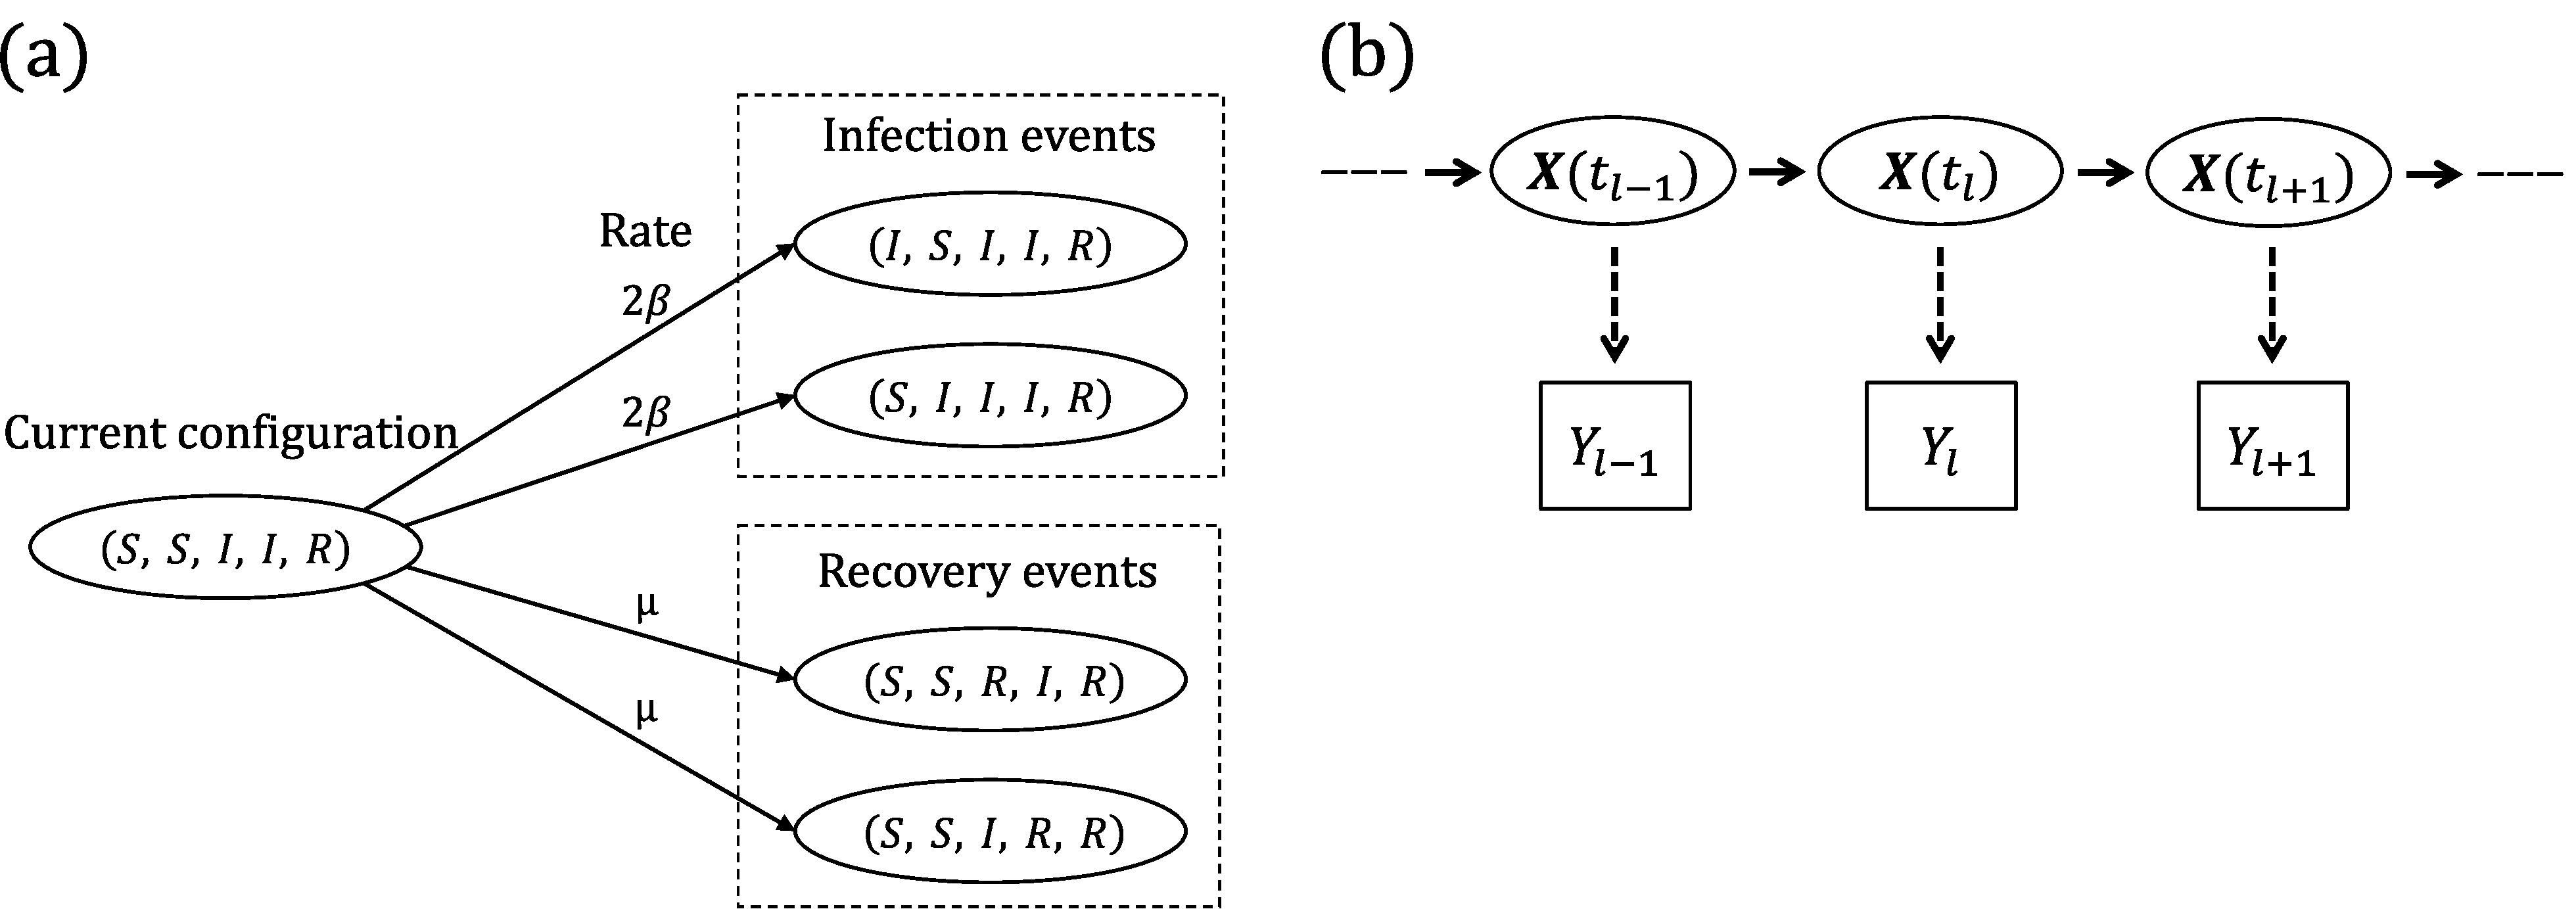
\includegraphics[width=0.95\linewidth]{figures/SIRdynamics_HMM}
	\caption[Diagram of subject--level state transitions and HMM structure for an SIR model.]{(a) SIR dynamics in a population of five subjects. The number of infecteds can increase from two to three via an infection of the first or second subject, reaching each of those configurations at rate $ 2\beta $. The number of recovered individuals can increase from one to two via a recovery of the third or fourth subject, reaching each of those configurations at rate $ \mu $. (b) Hidden Markov model for the joint distribution of the latent epidemic process and the data. The observations, $\mathbf{Y}_\ell,\ \ell=1,\dots,L$, are conditionally independent given $\bX(t)$, and $ \bY_\ell | I_{t_\ell}, \rho\sim\mathrm{Binomial}(I_{t_\ell}, \rho) $.}
	\label{fig:bda_SIRdynamics_HMM}
\end{figure}

\subsection{Subject--path proposal framework}
\label{subsec:bda_subj_proc}
The observed data likelihood in the posterior  $$ \pi(\btheta|\bY) \propto \pi(\bY|\btheta)\pi(\btheta)=\int L(\bY|\bX, \btheta) \pi(\bX|\btheta) \pi(\btheta) \mathrm{d}\pi(\bX)$$
is analytically intractable for even moderately sized $ N $ as it involves a  high dimensional integral over the collection of subject--paths, $ \bX $. The strategy employed in DA methods is to introduce the subject--paths, $ \bX $, as latent variables in the model. This enables us to work with the tractable complete data likelihood given by (\ref{eqn:bda_comp_data_likelihood}). The joint posterior distribution is \begin{equation}
\label{eqn:bda_jointpost}
\pi(\btheta, \bX| \bY) \propto \Pr(\bY|\bX,\rho) \times\pi(\bX|\bX(t_1),\beta,\mu) \times \Pr\left (\bX(t_1)|\bp_{t_1}\right) \times\pi(\beta)\pi(\mu) \pi(\rho) \pi(\bp_{t_1}),
\end{equation} where $ \pi(\beta)$, $\pi(\mu)$, $\pi(\rho)$, and $\pi(\bp_{t_1}) $ are prior densities. Our MCMC targets the joint posterior distribution, given by (\ref{eqn:bda_jointpost}), as we alternate between updating $ \bX|\btheta,\bY $ and $ \btheta|\bX,\bY $. 

Given the current collection of subject--paths, $ \xcur $, we propose $ \xnew $ by sampling the path of a single subject $\bX_j$, conditionally on the data, using a time--inhomogeneous CTMC with state space $ \mcS_j  $ and rates conditioned on the collection of disease histories of other individuals, $ \bx_{(-j)}  = \lbrace \bx_1,\dots,\bx_{j-1},\bx_{j+1},\dots,\bx_N \rbrace$. The proposed collection of paths is accepted or rejected in a Metropolis--Hastings step. 

Let $ \btau^{(j)} = \lbrace \tau_\mathrm{I}^{(j)},\tau_\mathrm{R}^{(j)}\rbrace $ be the (possibly empty) set of infection and recovery times for subject $ j $, and define $ \btau^{(-j)} = \lbrace\btau\setminus\btau^{(j)}\rbrace = \left \lbrace \tau_0^{(-j)} ,\tau_1^{(-j)}, \dots, \tau_{M}^{(-j)}, \tau_{M+1}^{(-j)}\right \rbrace$, where $ t_1 \equiv \tau_0^{(-j)} $ and $ t_L\equiv\tau_{M+1}^{(-j)} $, to be the set of $ M\leq K $ (ordered) times at which other subjects become infected or recover, along with $ t_1$ and $ t_L $. Let $ \mcI = \lbrace \mcI_1, \dots,\mcI_{M+1}\rbrace $ be the intervals that partition $ [t_1,t_L]$, i.e. $ \mcI_1 = \left [\tau_0^{(-j)},\tau_1^{(-j)}\right ),\ \mcI_2=\left [\tau_1^{(-j)},\tau_2^{(-j)}\right ),\dots,\ \mcI_{M+1}=\left [\tau_{M}^{(-j)},\tau_{M+1}^{(-j)}\right )$. Let $ I_\tau^{(-j)} = \sum_{i\neq j}\ind{\bX_i(\tau) = I} $ be the prevalence at time $ \tau $, excluding subject $ j $. Let $ \bLambda^{(-j)}(\btheta) = \left \lbrace\bLambda_1^{(-j)}(\btheta),\dots,\bLambda_{M+1}^{(-j)}(\btheta) \right \rbrace$ be the sequence of rate matrices corresponding to each interval in $ \mcI $, where for $ m=1,\dots,M+1 $,
\begin{equation} \bLambda_m^{(-j)}(\btheta) = \bordermatrix{ & S & I & R \cr
	S & -\beta I_{\tau_m}^{(-j)} & \beta I_{\tau_m}^{(-j)} & 0 \cr 
	I & 0 & -\mu & \mu \cr
	R & 0 & 0 & 0 }.
\end{equation}

We can construct the transition probability matrix for subject $ j $ over interval $ I_m $, $$ \bP^{(j)}(\tau_{m-1},\tau_m) = \left (
p_{a,b}^{(j)}(\tau_{m-1},\tau_m)\right )_{a,b\in \mcS_j}, $$ where $ p_{a,b}^{(j)}(\tau_{m-1},\tau_m) = \Pr(\bX_j(\tau_m)=b|\bX_j(\tau_{m-1})=a, \btheta) $, using the matrix exponential $$
	\bP^{(j)} (\tau_{m-1},\tau_m)= \exp\left [(\tau_m - \tau_{m-1})\bLambda^{(-j)}_m(\btheta)\right ].
	$$
This computation requires an eigen--decomposition of each rate matrix. We may reduce the total computational burden by computing the eigen decompositions analytically, and by caching the decompositions to avoid duplicate computations. One additional point is that while the eigenvalues of any SIR rate matrix are always real valued, this is not generally true, e.g., it is possible for the rate matrix of an SIRS model to have complex eigenvalues. In this case, we obtain a real valued transition probability matrix by first applying a rotation to each rate matrix with complex eigenvalues to obtain its real canonical form \cite{hirsch2013differential}. This is discussed in Section \ref{sec:mtx_exp}.

By the Markov property, the time--inhomogeneous CTMC density over the observation period $ [t_1,t_L] $, denoted $ \pi(\bX_j | \bx_{(-j)}, \btheta) \equiv \pi\left (\bX_j | \bLambda^{(-j)}(\btheta); \mathcal{I}\right ) $, can be written as a product of time--homogeneous CTMC densities over the inter--event intervals $ \mcI_1,\dots,\mcI_{M} $. Thus,
\begin{equation}
\label{eqn:subj_level_dens}
\pi\left (\bX_j | \bLambda^{(-j)};\mathcal{I}\right ) = \Pr(\bX_j(t_1) | \bp_{t_1}) \prod_{m=1}^{M}\pi\left (\bX_j  | \bx_j(\tau_{m-1}), \bLambda^{(-j)}_m(\btheta);\mcI_m\right ).
\end{equation} 
Similarly, the transition probability matrix over an interval $ \mathcal{I}_\ell = [t_{\ell-1},t_\ell] $ can be written as the product of transition probability matrices over the sub--intervals in $ \mathcal{I}_\ell $, within which the subject--level CTMC is time--homogeneous. Thus, the transition probability matrix over an inter--observation interval, $ \mcI_\ell = [t_{\ell-1}, t_\ell] $, partitioned by $ S $ transition events that define inter--event intervals with endpoints given by times $ t_{\ell-1} \equiv \tau_{\ell,0}^{(-j)} < \tau_{\ell,1}^{(-j)}<\dots<\tau_{\ell,S-1}^{(-j)}  < \tau_{\ell,S}^{(-j)} \equiv t_\ell $, is constructed as
\begin{equation*}\label{eqn:inhomog_tpmprod} \bP^{(j)}(t_{\ell - 1},t_\ell) = \prod_{s=1}^{S}\bP^{(j)}\left(\tau_{\ell,s-1}^{(-j)},\tau_{\ell,s}^{(-j)}\right) .\end{equation*}

The MCMC algorithm for constructing a subject--path proposal proceeds in three steps (Figure \ref{fig:sampling_diagram}):  
\begin{enumerate}[nolistsep]
	\item \textit{HMM step}: sample the disease state of the subject under consideration at the observation times, conditional on the data and disease histories of other subjects.
	\item \textit{Discrete time skeleton step}: sample the state at times when the time--inhomogeneous CTMC rates change, conditional on the states sampled in the HMM step. 
	\item \textit{Event time step}: sample the exact times of transition events conditional on the sequence of states sampled in the previous steps. 
\end{enumerate}

\begin{figure}[htbp]
	\centering
	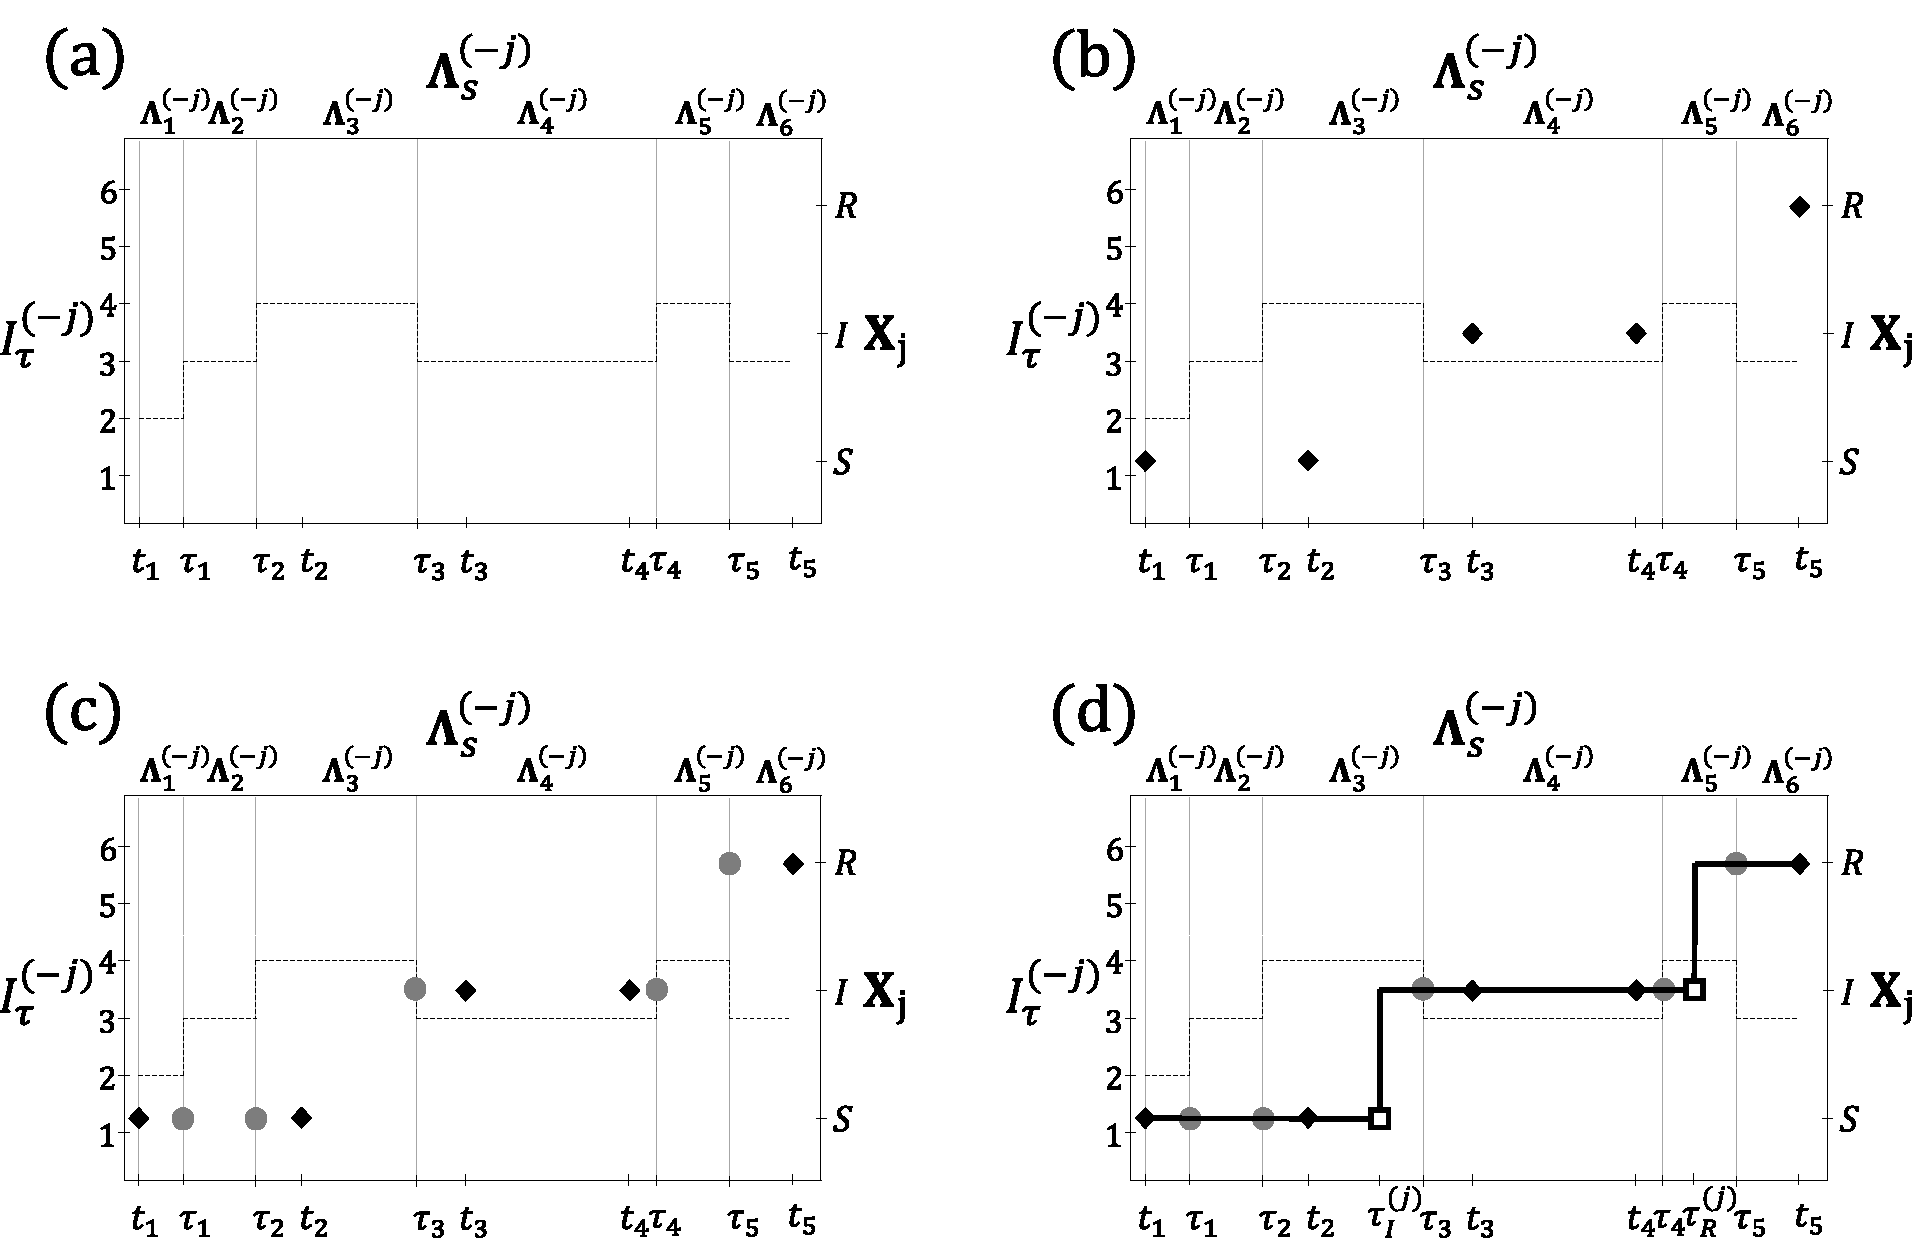
\includegraphics[width=0.95\linewidth]{figures/sampling_diagram.pdf}
	\caption[Diagram of subject--path proposals used in fitting models via Bayesian data augmentation.]{Procedure for constructing a subject--path proposal with SIR dynamics. (a) The dashed line depicts the number of infected individuals, excluding $ \bX_j $, the subject whose path is being sampled. The observation times, $ t_1,\dots,t_5 $, and times at which other subjects change disease states, $ \tau_1,\dots,\tau_5 $, are shown on the bottom axis. Rate matrices of the time--inhomogeneous CTMC (top axis) are constant within inter--event intervals (vertical lines). The state space of the subject--level process, $ \bX_j $, is shown on the right axis. (b) \textit{HMM step}: Sample the state of $ \bX_j $ at $ t_1,\dots,t_5 $, conditional on the data and on the disease histories of other subjects. (c) \textit{Discrete time skeleton step}: Sample the infection status at  $ \tau_1,\dots,\tau_5 $, conditional on the sequence of states sampled in the HMM step. (d) \textit{Event time step}: Sample the infection and recovery times from endpoint-conditioned time--homogeneous CTMC distributions, conditional on the sequence of disease states sampled in the HMM and discrete time skeleton steps.}
	\label{fig:sampling_diagram}
\end{figure}

\subsubsection{HMM step}
The key to sampling a sequence of disease states at the observation times is to rewrite the emission probability, given by (\ref{eqn:bda_emit_dist}), as
\begin{equation}\label{eqn:hmm_emit}
Y_\ell| X_j(t_\ell), I_{t_\ell}^{(-j)},\rho \sim \mathrm{Binomial}\left (\ind{X_j(t_\ell)=I} + I_{t_\ell}^{(-j)}, \rho\right ).
\end{equation}
If we treat the paths of all subjects except individual $ j $ as fixed, the emission probability in (\ref{eqn:hmm_emit}) only varies depending on whether subject $ j $ is infected at time $ t_\ell $. Furthermore, the data are conditionally independent of one another, given $ \bx$ and $ \btheta $, which induces a hidden Markov model (HMM) over the joint distribution $ \bX $ and $ \bY $ (Figure \ref{fig:bda_SIRdynamics_HMM}b). 

We sample the state of $ \bX_j $ at times $ t_1,\dots,t_L $ from the conditional distribution of $ \bX_j $, denoted $ \pi(\bX_j | \bY,\bx_{(-j)}, \btheta; t_1,\dots,t_L) $, using the stochastic forward--backward algorithm \cite{scott2002}. The algorithm enables us to efficiently sample from $ \pi\left (\bX \mid \bY, \bX_{(-j)}, \btheta\right ) $ by recursively accumulating, in a ``forward'' pass, information about the probability of various paths through $ \mcS $, conditional on the data, and then recursively sampling a trajectory in a ``backwards'' pass. 

In the forward recursion, we construct a sequence of matrices $ \bQ^{(t_2)}_j,\dots,\bQ^{(t_L)}_j $, where $ \bQ^{(t_\ell)}_j = \left (q_{j,r,s}^{(t_\ell)}\right )$, and $ q_{j,r,s}^{(t_\ell)} = \Pr\left (\bX_j(t_\ell) = s, \bX_j(t_{\ell - 1}) = r \mid \bY_{t_1}^{t_{\ell}},\bX_{(-j)},\btheta \right )$. Let $ \bP^{(j)}_{r,s}(t_{\ell - 1},t_\ell) = \Pr\left (\bX_j(t_\ell) = s \mid \bX(t_{\ell-1})=r, \btheta; \bX_{(-j)}\right ) $. If there are changes in the numbers of infected individuals in interval $ \mathcal{I}_\ell $, we construct the transition probability matrix for that interval as in (\ref{eqn:inhomog_tpmprod}). Then, 
\begin{equation}
q_{j,r,s}^{(t_\ell)} \propto \pi_{j}^{(t_\ell)}\left (r \mid \bX_{(-j)}, \btheta\right ) \times \bP^{(j)}_{r,s}\left (t_{\ell-1},t_\ell\right ) \times f\left (Y_{t_\ell} \mid \bX_j(t_\ell),\bX_{(-j)}(t_\ell), \rho, \bp_{t_1}\right ),	
\end{equation}
where $  \pi_{j}^{(t_\ell)}\left (r \mid \bX_{(-j)}, \btheta, \rho\right ) = \sum_r q_{j,r,s}^{(t_j)}$ and with proportionality reconciled via $ \sum_r\sum_s q_{j,r,s}^{(t_j)}=1 $.

In the backwards recursion, we sample the sequence of states at times $ t_1,\dots,t_L $ from the distribution $ \pi\left (\bX \mid \bY, \bX_{(-j)},\btheta, \rho,\bp_{t_1}\right )$. To do this, we first note that\vspace{-0.25in}

\begin{scriptsize}
	\begin{align*}\scriptsize
	\pi\left (\bX \mid \bY, \bX_{(-j)},\btheta, \rho,\bp_{t_1}\right ) &= \pi\left (\bX_j(t_L) \mid \bY_{t_1}^{t_L}, \bX_{(-j)},\btheta,\rho, \bp_{t_1}\right ) \prod_{\ell = 1}^{L-1}\pi \left (\bX_j(t_{L-\ell}) \mid \bX_{j,t_{L-\ell+1}}^{t_L}, \bX_{(-j)}, \bY_{t_1}^{t_L}, \btheta, \rho, \bp_{t_1}\right )\\
	&= \pi\left (\bX_j(t_L) \mid \bY_{t_1}^{t_L}, \bX_{(-j)},\btheta,\rho, \bp_{t_1}\right ) \prod_{\ell = 1}^{L-1}\pi \left (\bX_j(t_{L-\ell}) \mid \bX_{j,t_{L-\ell+1}}, \bX_{(-j)}, \bY_{t_1}^{t_{L-\ell+1}}, \btheta, \rho, \bp_{t_1}\right ),
	\end{align*}
\end{scriptsize} 
where the second equality follows from the conditional independence of the HMM. We proceed by first drawing $ \bX_j(t_L) $ from $ \pi_j^{(t_L)}\left (\cdot \mid \bX_{(-j)}, \btheta,\rho\right  ) $, and then drawing $ \bX_j(t_\ell),\ \ell = L-1,\dots,1, $ each in turn from the categorical distribution with masses proportional to column $ \bx_j(t_{\ell+1}) $ of $ \bQ_j^{(t_{\ell+1})} $. 

\subsubsection{Discrete-time skeleton step}
It would be straightforward to sample the exact infection and recovery times of subject $ j $, conditional on the sequence of states at times $ t_1,\dots, t_L $, if the subject--level CTMC rates did not possibly vary over each inter--observation interval. We may reduce our problem to the time--homogeneous case by first sampling the disease state at the intermediate event times when the CTMC rates change, and then sampling the full path within each inter--event interval. Consider an inter--observation interval, $ \mcI_\ell = [t_{\ell-1}, t_\ell] $, containing inter--event intervals whose endpoints are given by times $ t_{\ell-1} \equiv \tau_{\ell,0}^{(-j)} < \tau_{\ell,1}^{(-j)}<\dots<\tau_{\ell,n-1}^{(-j)}  < \tau_{\ell,n}^{(-j)} \equiv t_\ell $. We recursively sample $ \bX_j $ at each intermediate event time, beginning at $ \ttau_1 $, from the discrete distribution with masses 
\begin{align}
&\Pr\left (\bX_j\left (\ttau_{i}\right ) = x_{i} \mid  \bX_j\left (\ttau_{i-1}\right ) = x_{i-1}, \bX_j\left (\ttau_{n}\right ) = x_n\right ) \nonumber \\  &\hspace{1in}= \frac{\Pr\left (\bX_j\left (\ttau_{i}\right ) = x_{i}, \bX_j\left (\ttau_{i-1}\right ) = x_{i-1}, \bX_j\left (\ttau_{n}\right ) = x_n\right )}{\Pr\left (\bX_j\left (\ttau_{i-1}\right ) = x_{i-1}, \bX_j\left (\ttau_{n}\right ) = x_n\right )} \nonumber\\
&\hspace{1in}= \frac{\Pr\left (\bX_j\left (\ttau_{i}\right ) = x_{i} \mid \bX_j\left (\ttau_{i-1}\right ) = x_{i-1}\right )\Pr\left (\bX_j\left (\ttau_{n}\right ) = x_n \mid \bX_j\left (\ttau_{i}\right ) = x_{i}\right )}{\Pr\left (\bX_j\left (\ttau_{n}\right ) = x_n | \bX_j\left (\ttau_{i-1}\right ) = x_{i-1}\right)} \nonumber\\
&\hspace{1in} = \frac{\left [\bP^{(j)}\left (\ttau_{i-1},\ttau_{i}\right )\right ]_{x_{i-1},x_{i}}\left [\prod_{k=i}^{n-1}\bP^{(j)}\left (\ttau_{k}, \ttau_{k+1}\right )\right ]_{x_{i},x_n}}{\left [\prod_{k=i-1}^{n-1}\bP^{(j)}\left (\ttau_{k}, \ttau_{k+1}\right )\right]_{x_{i-1},x_n}}.
\label{eqn:dt_skel}
\end{align}

\subsubsection{Event time step}
The final step in constructing a subject--path is to sample the exact infection and recovery times given the discrete sequence of states obtained in the previous two steps. This amounts to simulating the path of an endpoint--conditioned time--homogeneous CTMC, a task for which there exist a variety of efficient methods \cite{hobolth2009}. When fitting the SIR model, we chose to use modified rejection sampling, a modification of Gillespie's direct algorithm \cite{gillespie1976general} that explicitly avoids simulating constant paths. This method is known to be efficient when the states differ at the endpoints of small time intervals. We used uniformization--based sampling \cite{hobolth2009} when fitting SEIR and SIRS models, which was more robust when sampling paths in intervals with multiple transitions. Fast implementations of these methods are available in the \texttt{ECctmc} package in \texttt{R} \cite{ECctmc}. We briefly summarize the algorithms below, and refer to \cite{hobolth2009} for a more thorough discussion.   

Our goal is to simulate a path for a time--homogeneous CTMC, $ \bX $, in the interval $ [0,T] $, conditional on $ \bX(0) = a $ and $ \bX(T) = b $. Let $ \bLambda $ be the rate matrix for the process. Let $ \Lambda_{a} $ denote the $ a,a $ diagonal element of $ \bLambda $, and similarly let $ \Lambda_{a,b} $ denote the rate given by the $ a,b $ element. We also denote by $ \mathbf{P}(T) $ the transition probability matrix for the CTMC over $ [0,T] $, and $ P_{ab}(T) $ the probability of beginning in state $ a $ and ending in state $ b $.

The modified rejection algorithm proposes paths by explicitly sampling the first transition time when it is known that at least one transition occurred (i.e. when $ a  \neq b $). The remainder of the path is proposed by forward sampling, using, for instance, Gillespie's direct algorithm. The proposed path is accepted if $ \bX(T) = b $. If a transition is not known to have occurred (i.e. when $ a = b $), a path is proposed via ordinary forward simulation and accepted if $ \bX(T) = b $. We sample the first transition time via the inverse--CDF method, sampling $ u\sim \mathrm{Unif}(0,1) $ and applying the inverse-CDF function 
\begin{equation} F^{-1}(u) = \frac{-log\left [1 - u \times \left (1 - \e^{-T\Lambda_a}\right )\right ]}{\Lambda_a}. 
\end{equation}

We found that the modified rejection algorithm worked well in fitting the SIR and SIRS models. In the examples we studied in which these models were fit, subject--paths over intervals where the endpoints required multiple jumps ($ S \rightarrow R $, or $ I \rightarrow S $) were almost never considered. Usually, only a single transition time was sampled in a given interval, so the inverse--CDF method was fast.

The uniformization algorithm samples the path for a time--homogeneous CTMC conditional on the state at the interval endpoints by coupling the original CTMC to the Markov chain for an auxilliary Poisson point process. State transitions, including virtual transition where the state does not change, are events of the point process, and the sequence of state labels is drawn from the corresponding Markov chain.

We construct the transition rate matrix of the auxilliary Markov chain, $ \bZ $, as $ R = I + \frac{1}{\mu}\bLambda $, where $ \mu = \max_a \bLambda_a$. The probability mass function for the number of state transitions, $ N $, conditional on $ \bX(0) = a,\ \bX(T) = b $, is
\begin{equation}
P(N=n|\bX(0) = a, \bX(T) = b) = \e^{-\mu T}\frac{(\mu T)^n}{n!}R_{ab}^n / P_{ab}(T).
\end{equation}
The algorithm proceeds by first sampling the number of state transitions from this distribution. If there are no transitions, or if there is one transition and the states at the endpoints are the same, the algorithm terminates. Otherwise, we drawn $ n $ independent uniform values in $ [0,T] $ and sort them to obtain the times of state transitions. The state labels at the sorted sequence of times, $ \tau_i $, $ i = 1,\dots,n-1 $, are drawn from the discrete distribution with masses given by
\begin{equation}
P(\bX(\tau_i) | \bX(\tau_{i-1}, \bX(T) = b) = \frac{R_{x_{i-1},x_i}(R^{n-i})_{x_ib}}{(R^{n-i+1})_{x_{i-1}b})}.
\end{equation}

Uniformization--based sampling was preferred in the case of the SEIR model since modified rejection sampling tended to get hung up when sampling paths in intervals where the endpoints suggested that at least two state transitions occured (which though it seldom occured, significantly slowed down the MCMC). We also note that the transition probability, $ P_{ab}(T) $, is computed and cached in executing the HMM step of our algorithm. Therefore, there are no additional eigen--decompositions or matrix exponentiations are required for the uniformization algorithm.

\subsubsection{Metropolis--Hastings step}
Having constructed a complete subject--path proposal, we decide whether to accept or reject it via a Metropolis--Hastings step. We emphasize that the true distribution of $ \bX_j | \bx_{(-j)},\btheta $ does not match the time--inhomogeneous CTMC in our proposal. Suppressing the dependence on $ \btheta $, the target distribution of the subject--path proposal is $ \pi(\bX | \bY) \propto\pi(\bY | \bX)\pi(\bX) $. Note that $ \xnew $ and $ \xcur $ differ only in the path of the $ j^{th} $ subject, so $ \Lambda^{(-j)}(\xcur) = \Lambda^{(-j)}(\xnew)=\bLambda^{(-j)} $.

Suppressing the dependence on $ \btheta$ for clarity, the acceptance ratio is
\begin{equation*}
a_{\xcur \longrightarrow \xnew} = \min \left \lbrace \frac{\pi(\xnew|\by)}{\pi(\xcur|\by)}\frac{q(\xcur|\xnew)}{q(\xnew|\xcur)},\ 1\right \rbrace
\end{equation*}

Now, \begin{eqnarray*}
	\pi(\xnew|\by) &\propto& \Pr(\by|\xnew)\pi(\xnew),\\
	\pi(\xcur|\by) &\propto& \Pr(\by|\xcur)\pi(\xcur),
\end{eqnarray*}

where $ \Pr(\by|\xnew) $ and $ \Pr(\by|\xcur )$ are binomial probabilities for the measurement process, and $ \pi(\xnew) $ and $ \pi(\xcur) $ are the time--homogenous CTMC densities of the current and the proposed population--level paths that appear in Equation (\ref{eqn:bda_comp_data_likelihood}). Let $ \pi(\xnew_j|\bLambda^{(-j)}; \mcI) $ and $ \pi(\xcur_j| \bLambda^{(-j)}; \mcI) $ denote the time--inhomogeneous subject--level CTMC proposal densities given by (\ref{eqn:subj_level_dens}). Then,
\begin{align*}
	q(\xnew|\xcur) &= \Pr(\xnew|\by; \bLambda^{(-j)}(\xcur), \mcI)\\
	&= \frac{\pi(\xnew, \by; \bLambda^{(-j)}(\xcur), \mcI)}{\Pr(\by; \bLambda^{(-j)}, \mcI)}\\
	&= \frac{\Pr(\by|\xnew)\pi(\xnew_j| \bLambda^{(-j)}; \mcI)}{\Pr(\by; \bLambda^{(-j)}(\xnew), \mcI)}\\
	\shortintertext{and similarly, } q(\xcur|\xnew) &= \frac{\Pr(\by|\xcur)\pi(\xcur_j| \bLambda^{(-j)}; \mcI)}{\Pr(\by; \bLambda^{(-j)}(\xcur), \mcI)}.
\end{align*}
Therefore, 
\begin{align*}
	\frac{\pi(\xnew|\by)}{\pi(\xcur|\by)}\frac{q(\xcur|\xnew)}{q(\xnew|\xcur)} &= \frac{\Pr(\by|\xnew)\pi(\xnew)}{\Pr(\by|\xcur)\pi(\xcur)}\frac{\Pr(\by|\xcur)\pi(\xcur_j; \bLambda^{(-j)})}{\Pr(\by|\xnew)\pi(\xnew_j; \bLambda^{(-j)})}\\
	&= \frac{\pi(\xnew)}{\pi(\xcur)}\frac{\pi(\xcur_j| \bLambda^{(-j)}; \mcI)}{\pi(\xnew_j| \bLambda^{(-j)}; \mcI)}.
\end{align*}
Hence the Metropolis--Hastings acceptance probability is
\begin{equation*}
a_{\xcur \longrightarrow\xnew}=\min \left \lbrace  \frac{\pi(\xnew)}{\pi(\xcur)}\frac{\pi(\xcur_j| \bLambda^{(-j)}; \mcI)}{\pi(\xnew_j| \bLambda^{(-j)}; \mcI)} , 1 \right \rbrace, 
\end{equation*}
which depends on the ratio is of the population-level time--homogeneous CTMC densities, multiplied by the ratio of time--inhomogeneous CTMC proposal densities. 

\subsubsection{Initializing the collection of subject--paths}
We initialize the collection of subject paths at the start of our MCMC by simulating paths using Gillespie's direct algorithm \cite{gillespie1976general} until we have found a path under which the data have non--zero probability. 
A sufficient condition for this under the binomial sampling model is that the number of infected individuals is greater than the observed prevalence at each observation time. 

\subsection{Parameter Updates and MCMC Scan Order}
\label{subsec:bda_mcmc_scan}
One MCMC iteration includes a number of subject--path updates, followed by a set of parameter updates. Conjugate priors were available for all parameters of the models in this chapter. Therefore, we chose to use Gibbs sampling to update parameter values from their univariate full conditional distributions (below).

There is no need to re--sample the path of every subject within each MCMC iteration. Indeed, we might suspect that the efficiency of our MCMC could be improved by sampling only a few subject--paths between parameter updates. Successive subject--path proposal tend to be highly autocorrelated, as with other DA methods \cite{roberts2001}, and are incur a relatively high computational cost. Frequently updating model parameters may help to break this correlation, despite the strong autocorrelations in posterior samples of model parameters. Often, the effective sample size (ESS) per CPU time is optimized by sampling only a handful of subject--paths per MCMC iteration. However, many factors, including the SEM dynamics, population size, efficiency of the implementation, and the degree of model misspecification could affect the optimal number subject--path updates per MCMC iteration. It is clearly impossible to disentangle all possible factors affecting the optimal number of subject--path updates per iteration. Therefore, we set the number of subject--paths per iteration on the basis of log--posterior ESS per CPU time in an initial run of 5,000--10,000 iterations.

\subsection{Data augmentation for SEIR dynamics}
\label{subsec:bda_seir_model}

The Susceptible--Exposed--Infectious--Recovered (SEIR) model adds a latent state to the SIR model in which subjects who are exposed to an infected individual incubate before becoming infectious. As with the SIR model, recovery is assumed to confer lifelong immunity. The structure of this model does not affect any of the machinery involved in the subject--path proposal mechanism, but rather merely redefines the population--level time--homogeneous CMTC for the epidemic process, and the subject--level time--inhomogeneous CTMC used in the subject--path proposals.

Under this model, we suppose that the data are sampled from a latent epidemic process, $ \bX = \lbrace \bX_1,\dots,\bX_N\rbrace $, that evolves in continuous--time as individuals become exposed, infectious, and recover. The state space of this process is $ \mcS = \lbrace S,E,I,R\rbrace^N $, the Cartesian product of $ N $ state labels taking values in $ \lbrace S,E,I,R\rbrace $. The state space of a single subject, $ \bX_j $, is $\mcS_j = \lbrace S, E, I, R\rbrace $, and a realized subject--path is of the form \begin{footnotesize}$ \bx_j(\tau) = \left (S,\ \tau < \tau^{(j)}_{\mathrm{E}};E,\  \tau^{(j)}_{\mathrm{E}} \leq \tau < \tau^{(j)}_{\mathrm{I}};I,\ \tau^{(j)}_{\mathrm{I}} \leq \tau < \tau^{(j)}_{\mathrm{R}};R\ ,\ \tau^{(j)}_{\mathrm{R}} \leq \tau
\right ) $\end{footnotesize}
where $ \tau^{(j)}_{\mathrm{E}} $, $ \tau^{(j)}_{\mathrm{I}} $, and $ \tau^{(j)}_{\mathrm{R}} $ are the times at which subject $ J $ becomes exposed, infectious, and recovers. As with the SIR model, some or all of these events may not transpire in the observation period $ [t_1,t_L] $, or at all. We let $ \beta $ be the per--contact infectivity rate, $ \gamma $ be the rate at which an exposed individual becomes infectious, and $ \mu $ be the rate at which an infectious individual recovers. Furthermore, we write the vector of disease state probabilities as $ \bp_{t_1} = (p_S,p_E,p_I,p_R) $. The latent epidemic process evolves according to a time--homogeneous CTMC, with transition rate from configuration $ \bx $ to $ \bx^\prime $ that differ only in the state of one subject $ j $ is given by $ \bLambda = \beta I $ if $ \bX_j = S $ and $ \bX^\prime_j = E$, $ \gamma $ if $ \bX_j = E $ and $ \bX^\prime_j = I$, and $ \mu $ if $ \bX_j = I $ and $ \bX^\prime_j = R$. Finally, the time--inhomogeneous CTMC rate matrices used in the subject--path proposal distribution have the form
\begin{equation} \bLambda_m^{(-j)}(\btheta) = \bordermatrix{ & S & E & I & R \cr
	S & -\beta I_{\tau_m}^{(-j)} & \beta I_{\tau_m}^{(-j)} & 0 & 0 \cr 
	E & 0 & -\gamma & \gamma & 0 \cr
	I & 0 & 0 & -\mu & \mu \cr
	R & 0 & 0 & 0 & 0 }.
\end{equation}
As with the SIR model, the eigenvalues of the CTMC rate matrices for the SEIR model are always real valued. The only computational modification, relative to the SIR model, that we suggest is that times of state transition in inter--event intervals be sampled conditional on the state at the endpoints via uniformization.

\subsection{Data augmentation for SIRS dynamics}
\label{subsec:bda_sirs_model}

The Susceptible--Infected--Recovered--Susceptible (SIRS) model modifies the SIR model to allow for loss of immunity. Again, fitting this model using our Bayesian data augmentation algorithm does not affect any of the machinery involved in the subject--path proposal mechanism, although the recurrent nature of the disease dynamics increases the computational burden since the disease state at the interval endpoints does not absolve us of sampling the full path within each inter--event interval where the states at the endpoints are the same.

Under the SIRS model, we suppose that the data are sampled from a latent epidemic process, $ \bX = \lbrace \bX_1,\dots,\bX_N\rbrace $, that evolves in continuous--time as individuals become exposed, infectious, and recover. The state space of this process is $ \mcS = \lbrace S,I,R\rbrace^N $, the Cartesian product of $ N $ state labels taking values in $ \lbrace S,I,R\rbrace $. The state space of a single subject, $ \bX_j $, is $\mcS_j = \lbrace S, I, R\rbrace $, and a realized subject--path is of the form\\ $ \bx_j(\tau) = \left (S,\ \tau < \tau^{(j)}_{\mathrm{I}_1}; 
	I,\ \tau^{(j)}_{\mathrm{I}_1} \leq \tau < \tau^{(j)}_{\mathrm{R}_1};
	R\ ,\ \tau^{(j)}_{\mathrm{R}_1} \leq \tau < \tau^{(j)}_{\mathrm{L}_1}; 
	S\ ,\ \tau^{(j)}_{\mathrm{L}_1} \leq \tau < \tau^{(j)}_{\mathrm{I}_2};\dots
	\right ) $,\\
where $ \tau^{(j)}_{\mathrm{I}_k} $, $ \tau^{(j)}_{\mathrm{R}_k} $, and $ \tau^{(j)}_{\mathrm{L}_k} $ are times at which subject $ J $ becomes infected, recovers, and loses immunity, and are ennumerated by the subscript $ k $ as the process may revisit each state multiple time. As with the SIR and SEIR models, it is possible that some or all of these events may not come about within the observation period $ [t_1,t_L] $. We let $ \beta $ be the per--contact infectivity rate, $ \mu $ be the rate at which an infectious individual recovers, and $ \gamma $ be the rate at which immunity is lost. We write the vector of disease state probabilities as $ \bp_{t_1} = (p_S,p_I,p_R) $. The latent epidemic process evolves according to a time--homogeneous CTMC, with transition rate from configuration $ \bx $ to $ \bx^\prime $ that differ only in the state of one subject $ j $ is given by $ \bLambda = \beta I $ if $ \bX_j = S $ and $ \bX^\prime_j = E$, $ \mu $ if $ \bX_j = I $ and $ \bX^\prime_j = R$, and $ \gamma $ if $ \bX_j = R $ and $ \bX^\prime_j = S$. Finally, the time--inhomogeneous CTMC rate matrices used in the subject--path proposal distribution have the form
\begin{equation} \bLambda_m^{(-j)}(\btheta) = \bordermatrix{ & S & I & R \cr
	S & -\beta I_{\tau_m}^{(-j)} & \beta I_{\tau_m}^{(-j)} & 0  \cr 
	I & 0 & -\mu & \mu \cr
	R & \gamma & 0 & -\gamma }.
\end{equation}
Unlike the SIR and SEIR models, eigenvalues of each CTMC rate matrix may be complex. In order to obtain a real valued transition probability matrix over an interval for which eigenvalues of the rate matrix are complex, we must rotate that rate matrix to obtain its real canonical form. This is further discussed in Section \ref{sec:mtx_exp}.

\section{Simulation results}
\label{sec:bda_simulations}

\subsection{Inference Under a Variety of Epidemic Dynamics}
\label{subsec:bda_sir_seir_sirs_sim}
We fit SIR, SEIR, and SIRS dynamics to binomially distributed prevalence counts sampled from epidemics simulated under corresponding dynamics in populations of 750, 500, and 200 individuals (details provided in Section \ref{sec:bda_sim1_details}). Priors for the rate parameters and binomial sampling probability were chosen so that the priors spanned reasonable ranges of values (e.g. recovery durations ranging from days to weeks/months rather than seconds to eons under extremely diffuse priors), but were otherwise only mildly informative, while the initial distribution parameters were assigned informative priors (see tables \ref{tab:sim1_sir_priors}, \ref{tab:sim1_seir_priors}, and \ref{tab:sim1_sirs_priors}). The three datasets, depicted in Figure \ref{fig:sim1_latent_posts} along with the estimated pointwise posterior prevalence, presented a range of challenges. The SIR example was arguably the most ``standard'' example as the observation period captured the exponential growth and decline of the epidemic. Thus, much of the curvature in the latent path was reflected in the data. In contrast, data from the outbreak simulated under near--endemic SEIR dynamics contained very little information about the shape of the epidemic curve. The task of disentangling whether the data were sampled with low probability from a high--prevalence outbreak, or visa--versa, was further complicated by the inclusion of an additional disease state --- the exposed state --- that was not directly observed. Finally, the SIRS model was more computationally challenging for two reasons. First, the recurrent nature of the disease process demanded that the disease state at each event time, and the path within each inter--event interval, be sampled in the subject--path proposal. Second, it was possible for CTMC rate matrices to have complex eigen--decompositions, which made computing transition probability matrices more expensive. This affected the optimal number of subject--path updates per MCMC iteration (see Section \ref{sec:num_subj_per_iter} for further discussion of this point).

\begin{figure}[!h]
	\centering
	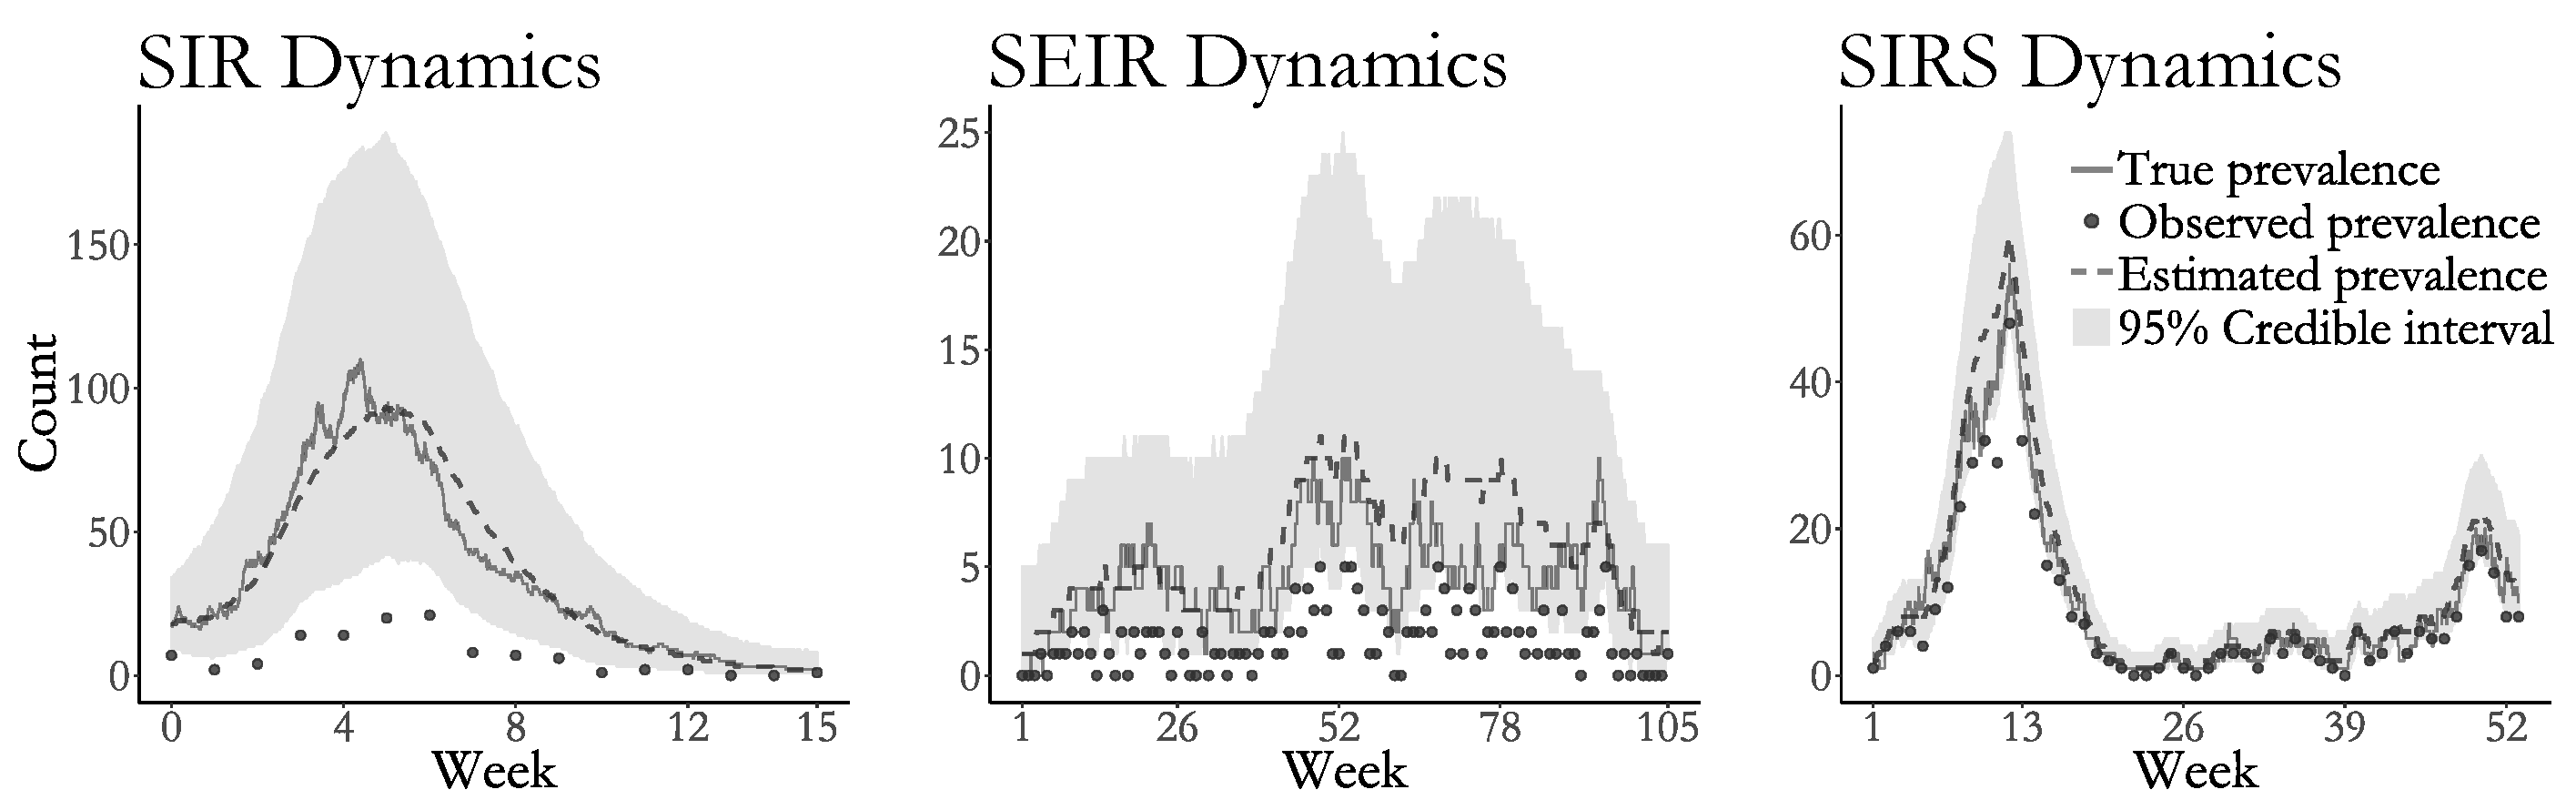
\includegraphics[width=\linewidth]{figures/sim1_latent_posts.pdf}
	\caption[Estimated latent posteriors for SIR, SEIR, and SIRS models fit to simulated prevalence data.]{Estimated latent posterior distributions of disease prevalence in outbreaks simulated under SIR (left), SEIR (middle), and SIRS (right) dynamics. Depicted are the true unobserved prevalence (solid line), observed data (dots), pointwise posterior median prevalence (dashed line), and pointwise 95\% credible intervals (shaded region). Latent posterior estimates are based on a thinned sample, with every $250^{th}$ sample retained.}
	\label{fig:sim1_latent_posts}
\end{figure}

The true epidemic paths and parameter values fell well within the 95\% Bayesian credible intervals in all three simulations (Figure \ref{fig:sim1_latent_posts} presents the estimated latent posterior prevalence; Figure \ref{fig:sim1_credint} presents posterior estimates of model parameters; Figure \ref{fig:sim1_latent_post_all} presents estimated latent posterior distributions and true epidemic paths for all model compartments). The acceptance rates for subject--path proposals were roughly 92\% for the SIR model, 91\% for the SEIR model, and 77\% for the SIRS model. Our posterior estimates of the model parameters also closely match estimates obtained using the particle marginal Metropolis--Hastings (PMMH) algorithm of \cite{andrieu2010particle}, implemented using the \texttt{pomp} package in \texttt{R} \cite{pomp}. We simulated particle paths in the PMMH algorithm in two ways; exactly using Gillespie's direct algorithm \cite{gillespie1976general}, and approximately using a multinomial modification of $ \tau $--leaping \cite{breto2011compound}. In these small population examples, the exact algorithm is arguably more appropriate, as the leap conditions for $ \tau $--leaping may not be met in small populations, but it is also substantially slower. In these simple settings, PMMH tended to outperform our algorithm in terms of log--posterior effective sample size (ESS) per CPU time. When PMMH particle paths were simulated by $ \tau $--leaping, the average ESS per CPU compared to BDA was roughly $ 350\times $ greater for the SIR model, $ 4.4\times $ greater for the SEIR model, and $ 13\times $ greater for the SIRS model. Exact simulation of PMMH particle paths reduced the computational advantage of PMMH substantially. In this case, the average log--posterior ESS per CPU time was $ 10.5\times $ greater for PMMH in fitting the SIR model, $ 2\times $ for the SEIR model, and $ 0.7\times $ for the SIRS model. These comparisons did not include the time required to tune the MCMC for PMMH, which was nontrivial. In contrast, our algorithm required no tuning beyond selecting the number of subject--paths to update per MCMC iteration. We also note that in fitting the models using PMMH, we were required to make several implementation decisions to prevent particle degeneracy and to balance speed with precision. These included selecting the number of particles and the time--step in the approximate $ \tau $--leaping algorithm. For example, when using $ \tau $--leaping to simulate particle paths, the number of particles required to obtain good mixing for the SIRS model fit with PMMH was much higher than for the other two models. Details of the PMMH implementations and further results are discussed in Section \ref{sec:bda_sim1_details}.

\begin{figure}[!h]
	\centering
	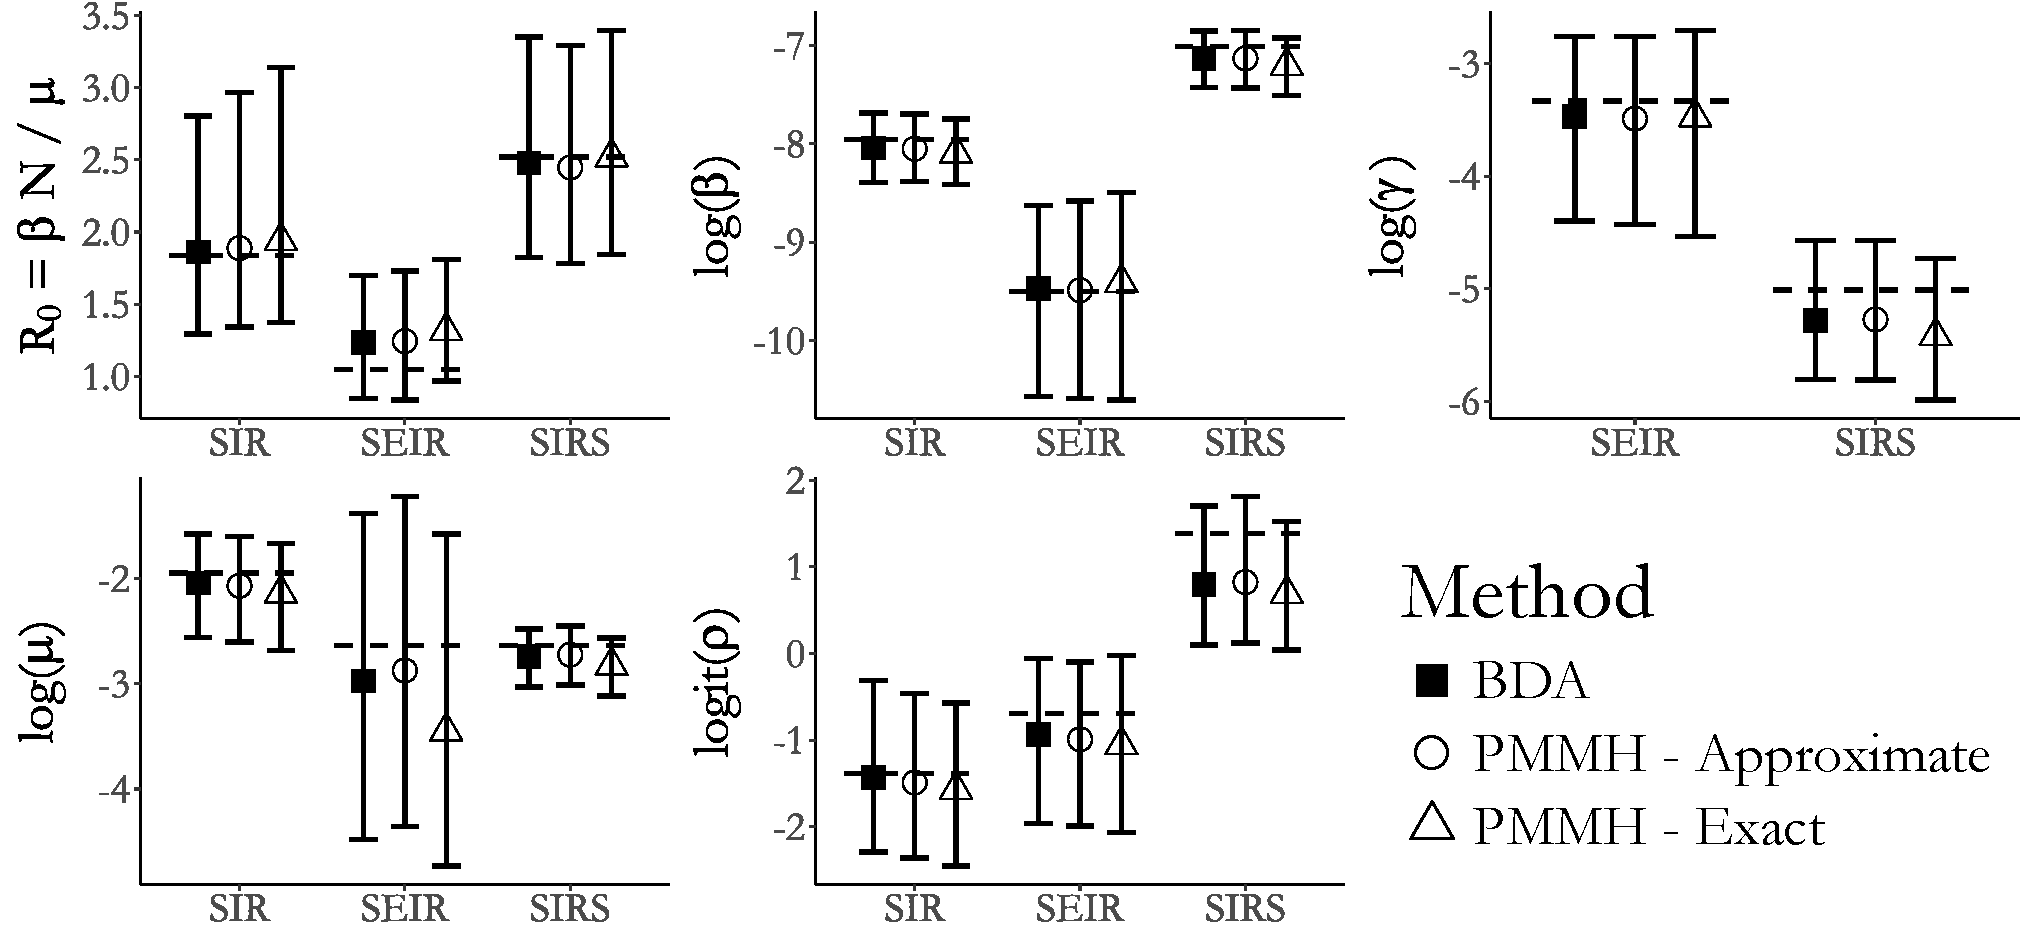
\includegraphics[width=\linewidth]{figures/sim1_credints.pdf}
	\caption[Posterior estimates of SIR, SEIR, and SIRS model parameters fit to simualted data using Bayesian data augmentation and PMMH.]]{Posterior medians and 95\% credible intervals of parameters in the SIR, SEIR, and SIRS models fit with Bayesian data augmentation (BDA) and particle marginal Metropolis--Hastings (PMMH) with particle paths simulated approximately (using $ \tau $--leaping) and exactly (using Gillespie's direct algorithm). Displayed are estimates of the basic reproductive number, $ R_0 $, the rate parameters, and the binomial sampling probability. In all models, $ \beta $ is the per--contact infectivity rate, $ \mu $ is the recovery rate, and $ \rho $ is the binomial sampling probability. In the SEIR model, $ \gamma $ denotes the rate at which an exposed individual becomes infectious, while in the SIRS model $ \gamma $ denotes the rate at which immunity is lost.}
	\label{fig:sim1_credint}
\end{figure}

\subsection{Inference under model misspecification}
\label{subsec:bda_misspec_sim}
In practice, every stochastic epidemic model is misspecified with respect to the real world epidemic process from which the data arise, and the malignancy of the model misspecification is often imposible to diagnose a priori. We can build up an understanding of an epidemic's dynamics by fitting SEMS under a range of dynamics, beginning with simple, easily interpretable models. The results of each model are interpretted counterfactually --- e.g. ``If the true epidemic followed SIR dynamics, our best guess of the dynamics that gave rise to the data would be...''. The iterative nature of epidemic modeling suggests that some minimal criteria for the usefulness of any computational algorithm would be that, for a reasonable model, the MCMC should converge to the posterior of the model parameters, and that the estimated latent posterior distribution under the hypothetical dynamics should reflect the true epidemic.

However, it is precisely the inherent misspecification of SEMs that leads simulation--based methods to struggle in many instances, and it is here that we highlight a critical advantage of our DA algorithm. Our subject--path proposals are driven, not just by the SEM dynamics, but also by the data. This enables us to overcome model misspecification when simulation--based methods degenerate due to their reliance on an adequately accurate model for simulating epidemic paths. We demonstrate this in a simple example in which we fit SIR and SEIR models to four years of weekly prevalence data sampled from an epidemic simulated under time--varying SEIR dynamics, where the latent period, infectious period, and per--contact infectivity rate were modulated over four discrete epochs (depicted in Figure \ref{fig:misspec_data}, details presented in Section \ref{sec:bda_misspec_sim_details}).

\setcounter{table}{1}
\begin{figure}[!ht]
	\centering
	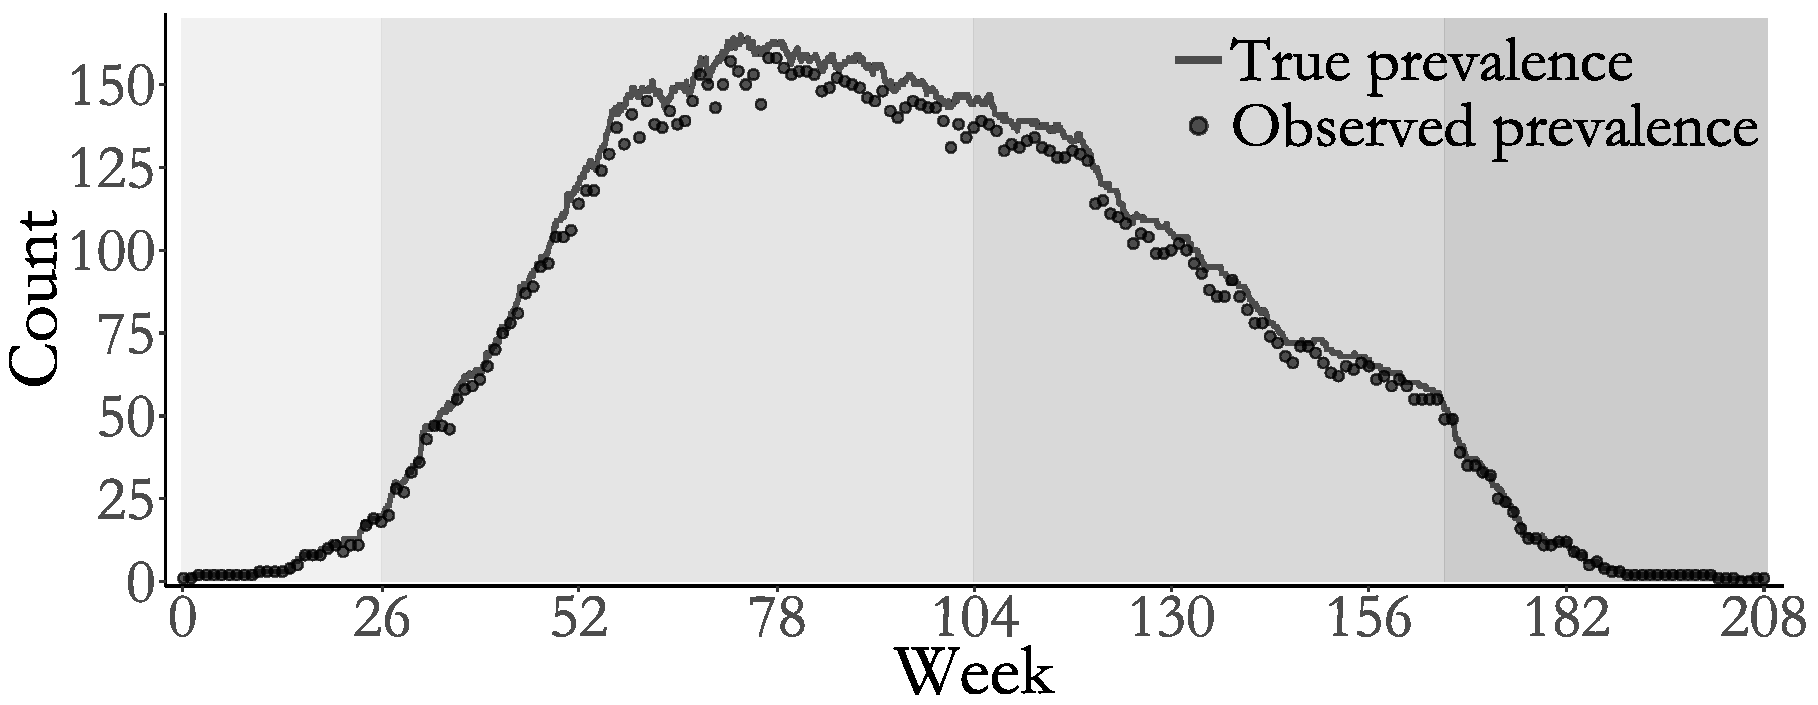
\includegraphics[width=0.5\linewidth]{figures/SEIR_misspec_data.pdf}
	\qquad
	\begin{tabular}[b]{lllll}
		& \multicolumn{4}{c}{Epoch}\\ \cmidrule{2-5}
		Parameter & 1 & 2 & 3 & 4 \\ \hline	
		$ R_0^{\mathrm{Eff}} $ & 14.9& 9.2& 0.1& 0\\
		$ 1/\gamma $ (days) & 210&210&90& 180\\
		$ 1/\mu $ (days) & 150 &330&300&70	\\
		&&&&
	\end{tabular}
	\captionsetup{labelformat=andtable}
	\caption[Simulated outbreak data from an SEIR model with time--varying dynamics.]{Simulated outbreak with SEIR dynamics that varied over four epochs (shaded regions). Weekly prevalence counts (points) were binomially sampled with sampling probability $ \rho = 0.95 $ from the true unobserved prevalence (solid line). The table presents the effective reproductive number computed based on the number of susceptibles at the beginning of each epoch, $ R_0^{\mathrm{Eff}} = \beta(\tau) S(\tau) / \mu(\tau) $, the mean latent period, $ 1/\gamma $, and the mean infectious period, $ 1/\mu $.}
	\label{fig:misspec_data}
\end{figure}

We fit SIR and SEIR models using our DA algorithm, and using PMMH with 2,500 particles, the paths for which were simulated approximately via $ \tau $--leaping with a time--step of 1 day. We assigned weakly informative priors for the rate parameters governing the epidemic dynamics in both models, and informative priors for the binomial sampling probability and the initial state probabilities (Table \ref{tab:misspec_priors}). MCMC chains for models fit via PMMH were plagued by particle degeneracy and did not converge (Figures \ref{fig:misspec_sir_bda_traceplots} and \ref{fig:misspec_seir_bda_traceplots}).

Both models fit via DA yield reasonable estimates for the within--subject disease dynamics (i.e. the infectious period, as well as the latent period in the case of the SEIR model). The posterior median average infectious period duration was estimated to be 292 days (95\% BCI: 263 days, 323 days) under SIR dynamics, and 287 days (95\% BCI: 260 days, 318 days) under SEIR dynamics. The posterior median average latent period under SEIR dynamics was 211 days (95\% BCI: 165 days, 260 days). The posterior median estimate of $ R_0 $ under SIR dynamics was 4.05 (95\% BCI: 3.40, 4.81), while under SEIR dynamics, the posterior median estimate of $ R_0 $ was 23.8 (95\% BCI: 15.1, 37.0). While the true prevalence fell well within the pointwise 95\% credible interval for both models (Figure \ref{fig:misspec_latent_posts}), we notice that the degree of model misspecification drastically affected our ability to estimate the history of the numbers of noninfectious people over the course of the epidemic. Under SIR dynamics, we drastically overestimate the number of susceptible individuals. The SEIR model much more closely resembles the time--varying SEIR model used to simulate the epidemic. Although the true path for the number of susceptible still falls outsize the 95\% credible interval at times, we are still able to reconstruct a reasonabe range of paths for the number of exposed individuals. This contrasts with the models fit in Section \ref{subsec:bda_sir_seir_sirs_sim}, which were not misspecified with respect to the true epidemic dynamics. In that case, the complete path of the epidemic fell well within the estimated credible intervals for all disease states for all three models (Figure \ref{fig:sim1_latent_post_all}). Therefore, we advise caution in  reconstructing the epidemic history for disease states that were not measured, particularly when severe model misspecification is suspected.

\begin{figure}[!h]
	\centering
	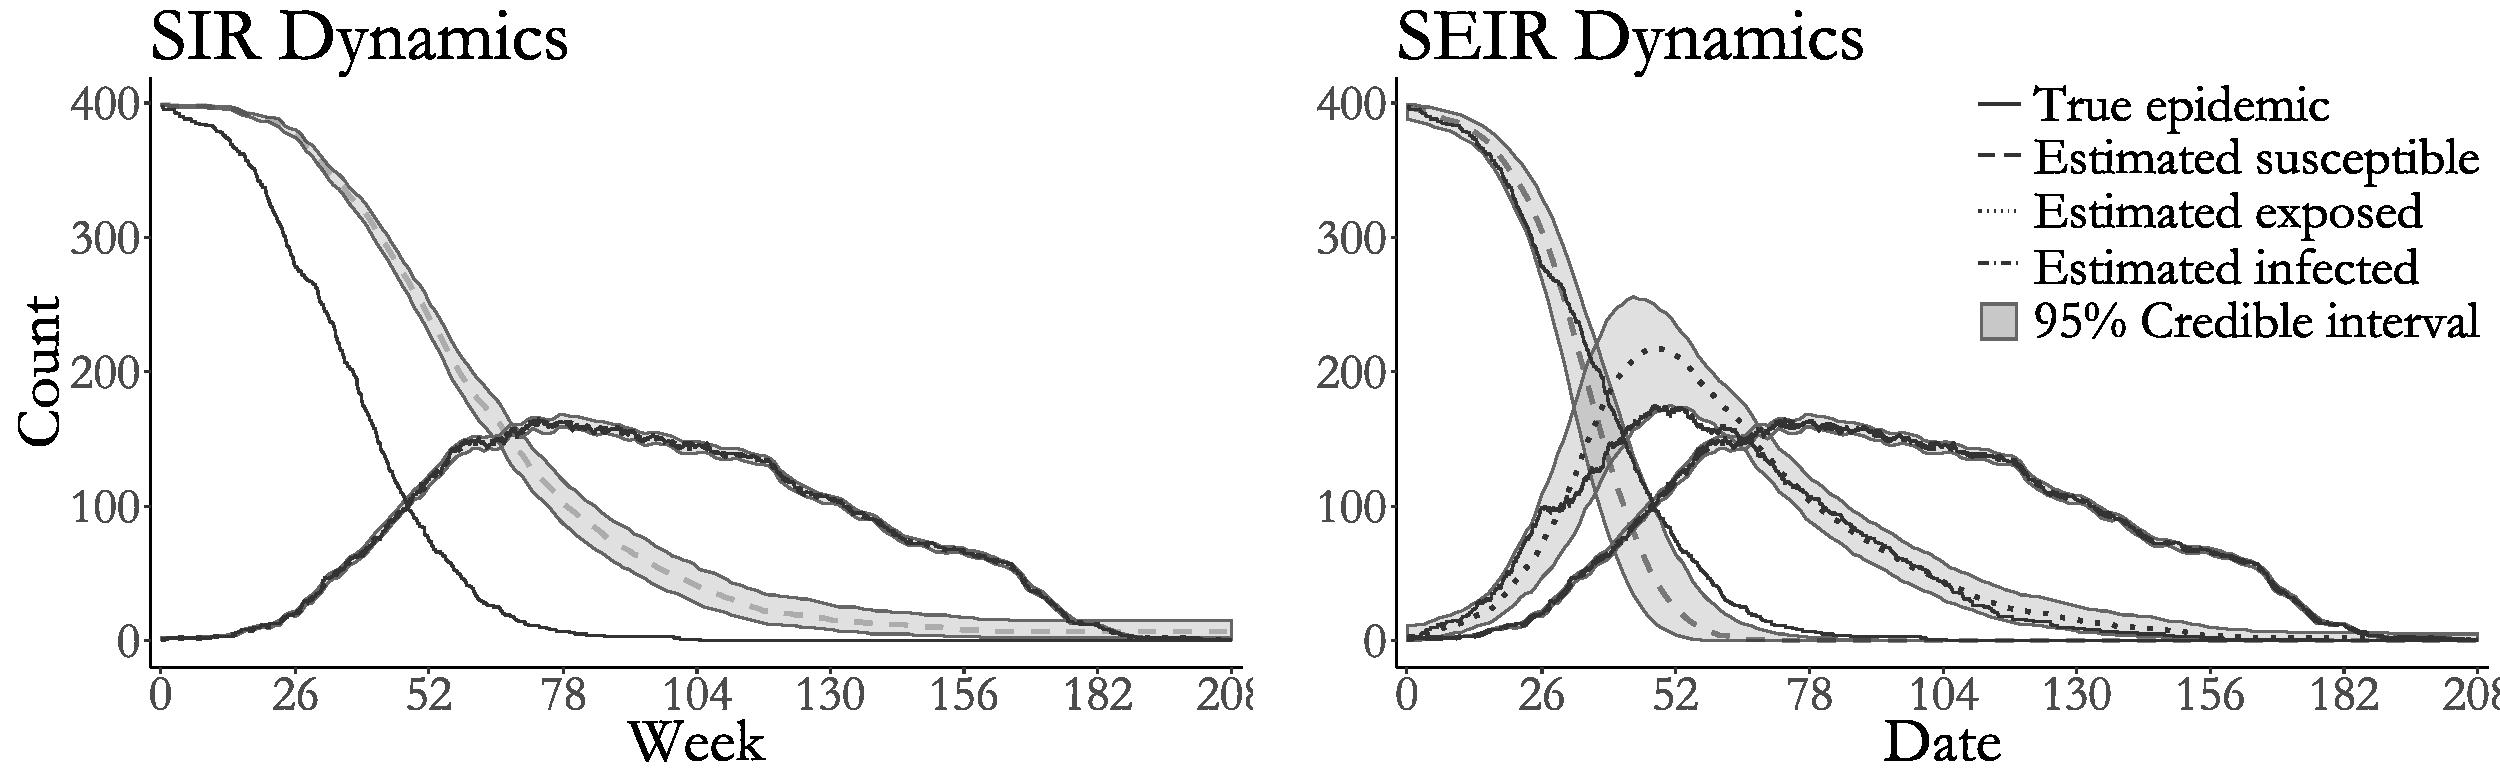
\includegraphics[width=0.9\linewidth]{figures/misspec_latent_posts.pdf}
	\caption[Latent posterior distributions for SIR and SEIR models fit to simulated data from an SEIR model with time--varying dynamics.]{True epidemic path (solid lines), pointwise posterior median estimate of the numbers of susceptibles (dashed line), exposed (dotted line), and infected individuals (dash--dotted line) and pointwise 95\% credible intervals (shaded regions) under SIR and SEIR dynamics.}
	\label{fig:misspec_latent_posts}
\end{figure}

\subsection{Effect of prior specification on posterior inference}
\label{subsec:prior_effect_sim}
Given the limited extent of aggregated prevalence counts, we must consider how our choices of prior distributions influence our posterior inferences. We simulated an outbreak with SIR dynamics in a population of 750 individuals for which $ R_0 = \beta \times 763 / \mu \approx 1.84 $ and the mean infectious period was $ 1/\mu = 7 $ days. We fit SIR models to binomially distributed weekly prevalence data, sampled with detection probability $ \rho = 0.2$, under the following four prior regimes: Regime 1 --- informative priors for all model parameters; Regime 2 --- vague priors for the rate parameters and an informative prior for the sampling probability; Regime 3 --- informative priors for the rate parameters and a flat prior for the sampling probability; Regime 4 --- vague priors for the rate parameters and a flat prior for the sampling probability. The same prior for the initial state probabilities was used in all four regimes. Complete simulation details and convergence diagnostics are supplied in Section \ref{sec:prior_effect_details}.

\begin{figure}[htbp]
	\centering
	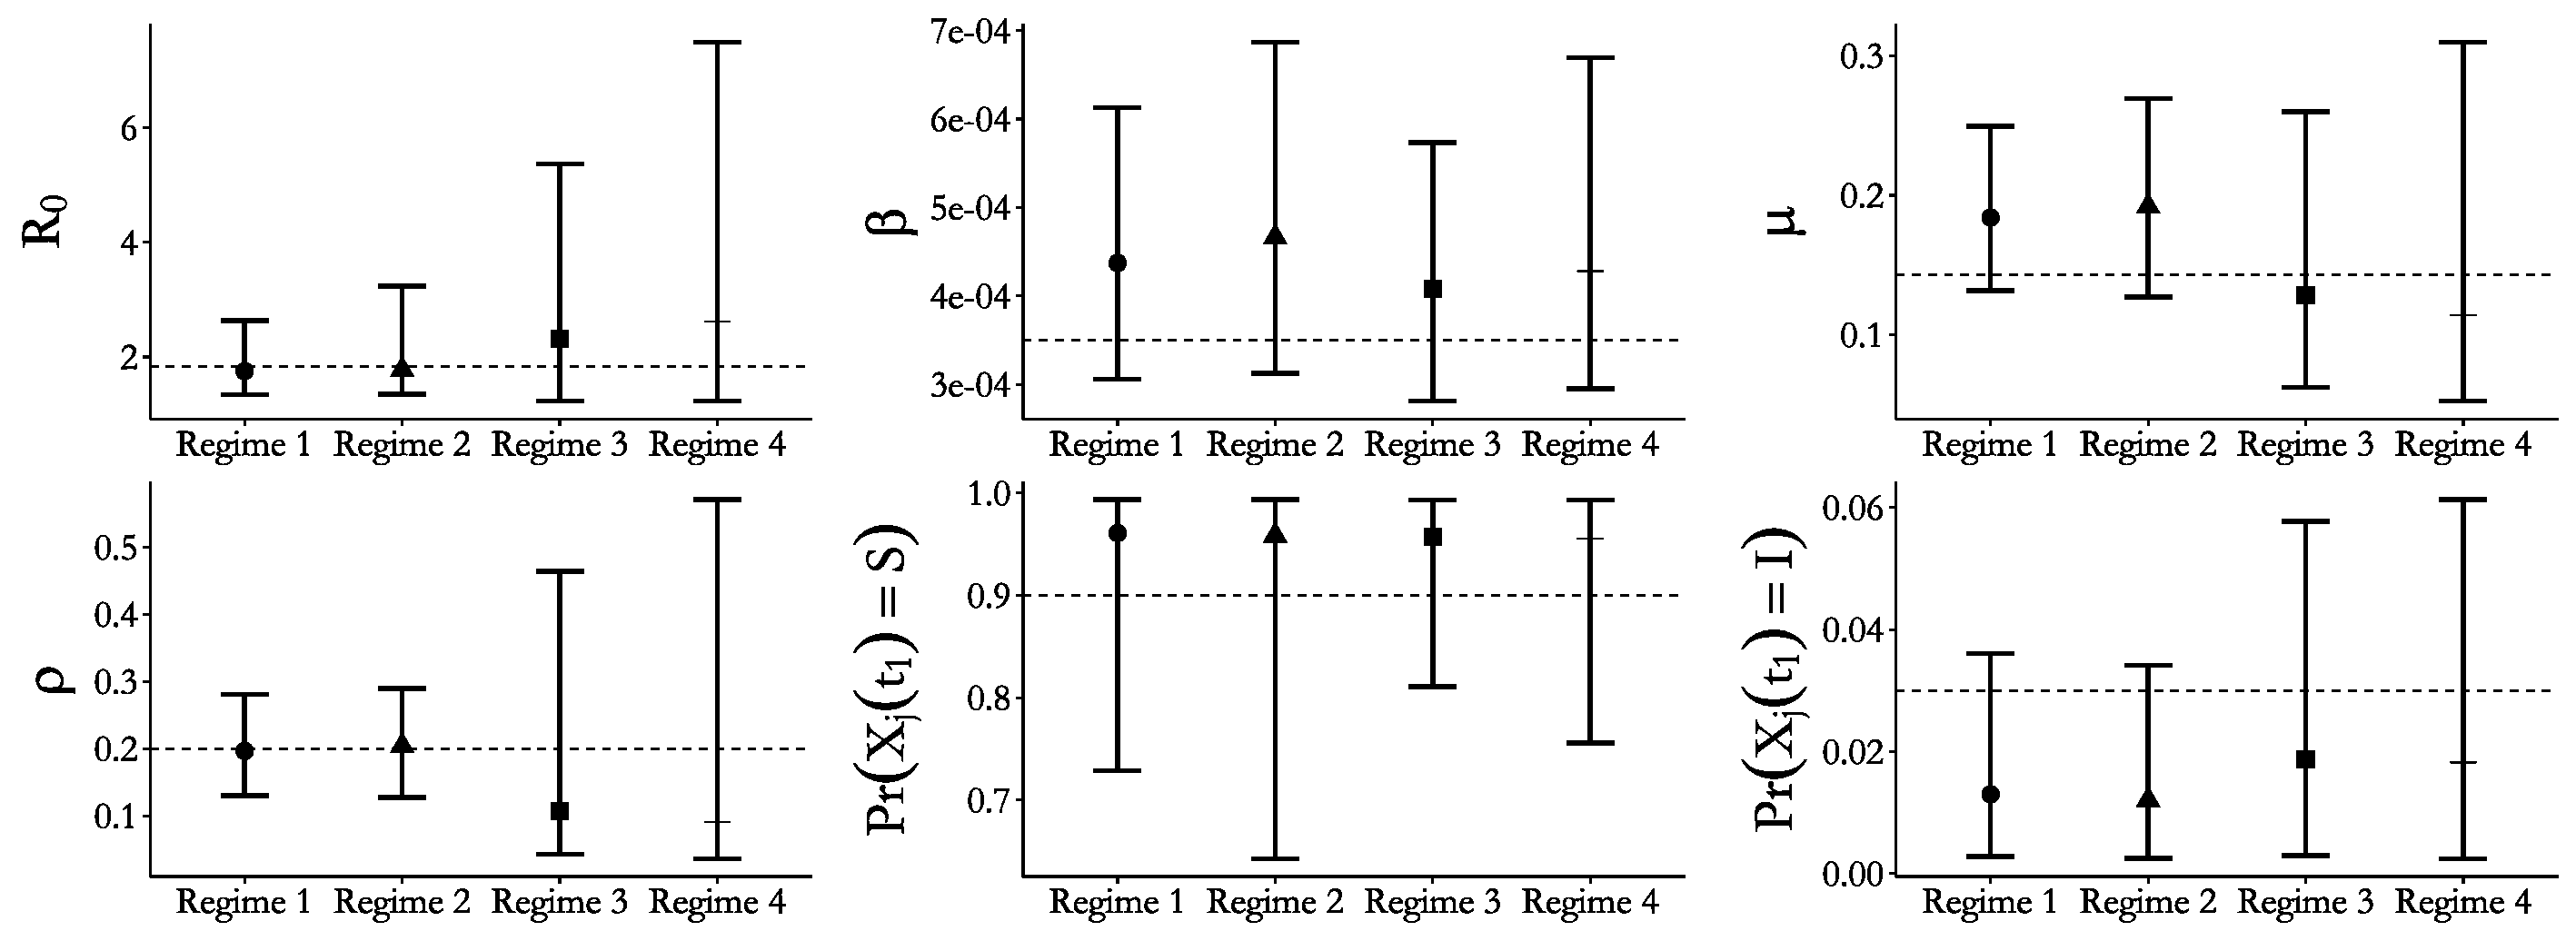
\includegraphics[width=\linewidth]{figures/prior_effect_credints.pdf}
	\caption[Posterior estimates of SIR model parameters under four prior regimes.]{Posterior median estimates and 95\% credible intervals for all SIR model parameters under four different prior regimes (Table \ref{tab:prior_effect_priors}). Regimes 1 and 3 set informative priors for the per--contact infectivity and recovery rates. Regimes 1 and 2 set informative priors for the binomial sampling probability. The same mildly informative prior for the initial state probabilities was used in all four regimes.}
	\label{fig:prior_credints}
\end{figure}

The true values for all model parameters fell within the 95\% credible intervals under all four prior regimes. Unsurprisingly, informative priors tended to result in narrower credible intervals for the parameters (Figure \ref{fig:prior_credints}) as well as for the latent process (Figure \ref{fig:prior_latent_posts}). The strength of prior information about the sampling probability affected the widths of credible intervals to a much greater extent than the priors for the rate parameters. Strong prior information about the sampling probability also resulted in substantially narrower credible intervals for disease prevalence under each of the prior regimes for the rate parameters. In contrast, informative priors for the rate parameters yielded only slightly narrower credible intervals for disease prevalence when holding constant the strength of the sampling probability prior. The effects on the initial state probability parameters seem to reverse this pattern, although we caution against overinterpretion given the paucity of data available for estimating those parameters. MCMC chains with strong priors for the binomial sampling probability also appeared to mix somewhat better than chains with diffuse priors for the sampling probabilty (see traceplots in Section \ref{sec:prior_effect_details}).

\begin{figure}[htbp]
	\centering
	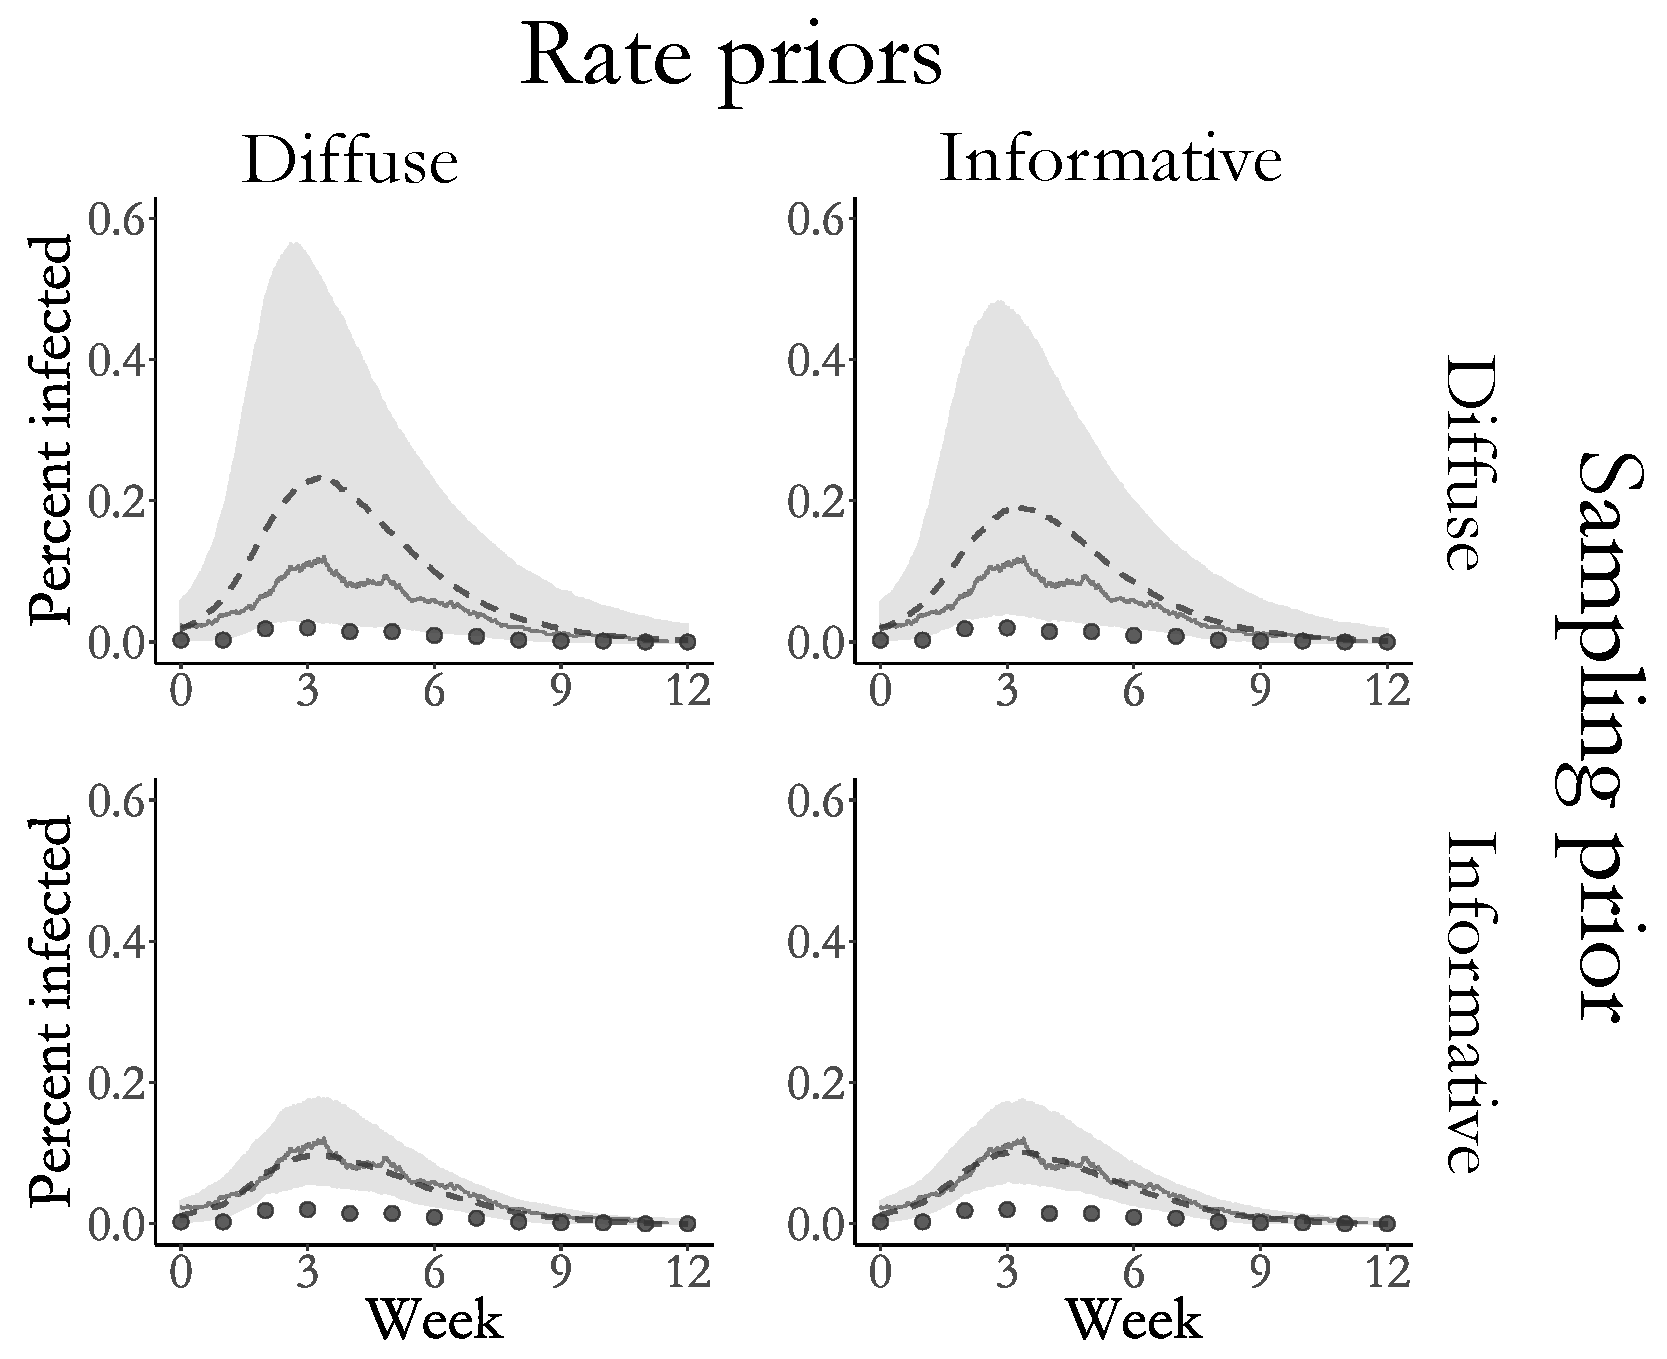
\includegraphics[width=0.6\linewidth]{figures/prior_latent_posts.pdf}
	\caption[Estimated latent posterior for an SIR model under four prior regimes.]{Estimated latent posterior distributions of disease prevalence in outbreaks simulated under four prior regimes for SIR model rate parameters and the binomial sampling probability. Depicted are the true unobserved prevalence (solid line), observed data (dots), pointwise posterior median prevalence (dashed line), and pointwise 95\% credible intervals (shaded region). Latent posterior estimates are based on a thinned sample, with every $250^{th}$ sample retained.}
	\label{fig:prior_latent_posts}
\end{figure}

\section{Example: Influenza in a British boarding school}
\label{sec:bda_bbs}

As an application, we analyze data from an outbreak of influenza in a British boarding school \citep{anon1978, davies1982}. This outbreak took place shortly after the Easter term began in January 1978, and was estimated to eventually infect roughly 90\% of the 763 boys aged 10--18. Daily counts of the boys who were confined to the infirmary from January $22^{nd}$ through February $4^{th}$ were accessed via the \texttt{pomp} package in \texttt{R} \citep{pomp}, and are displayed in Figure \ref{fig:bbs_dat}. 

We used our DA algorithm and PMMH to fit SIR and SEIR models with a binomial emission distribution to the data (see Section \ref{sec:bbs_supp} of the supplement for complete details). All of the parameters were assigned diffuse priors, which are plotted over the posterior ranges in Figure \ref{fig:bbs_densities}. The PMMH algorithm failed to converge for both models, which we suspect was due to a combination of model misspecification and the constrained state space of the binomial measurement process. We also fit a set of supplementary SIR and SEIR models in Section \ref{sec:bbs_neg_binom}, in which we assumed a negative--binomial emission distribution. This was done in order to facilitate comparison with PMMH, although we feel that a negative binomial emission distribution is not appropriate in such a closely monitored outbreak setting since it does not rule out over--reporting of cases.

\begin{figure}[ht!]
	\centering
	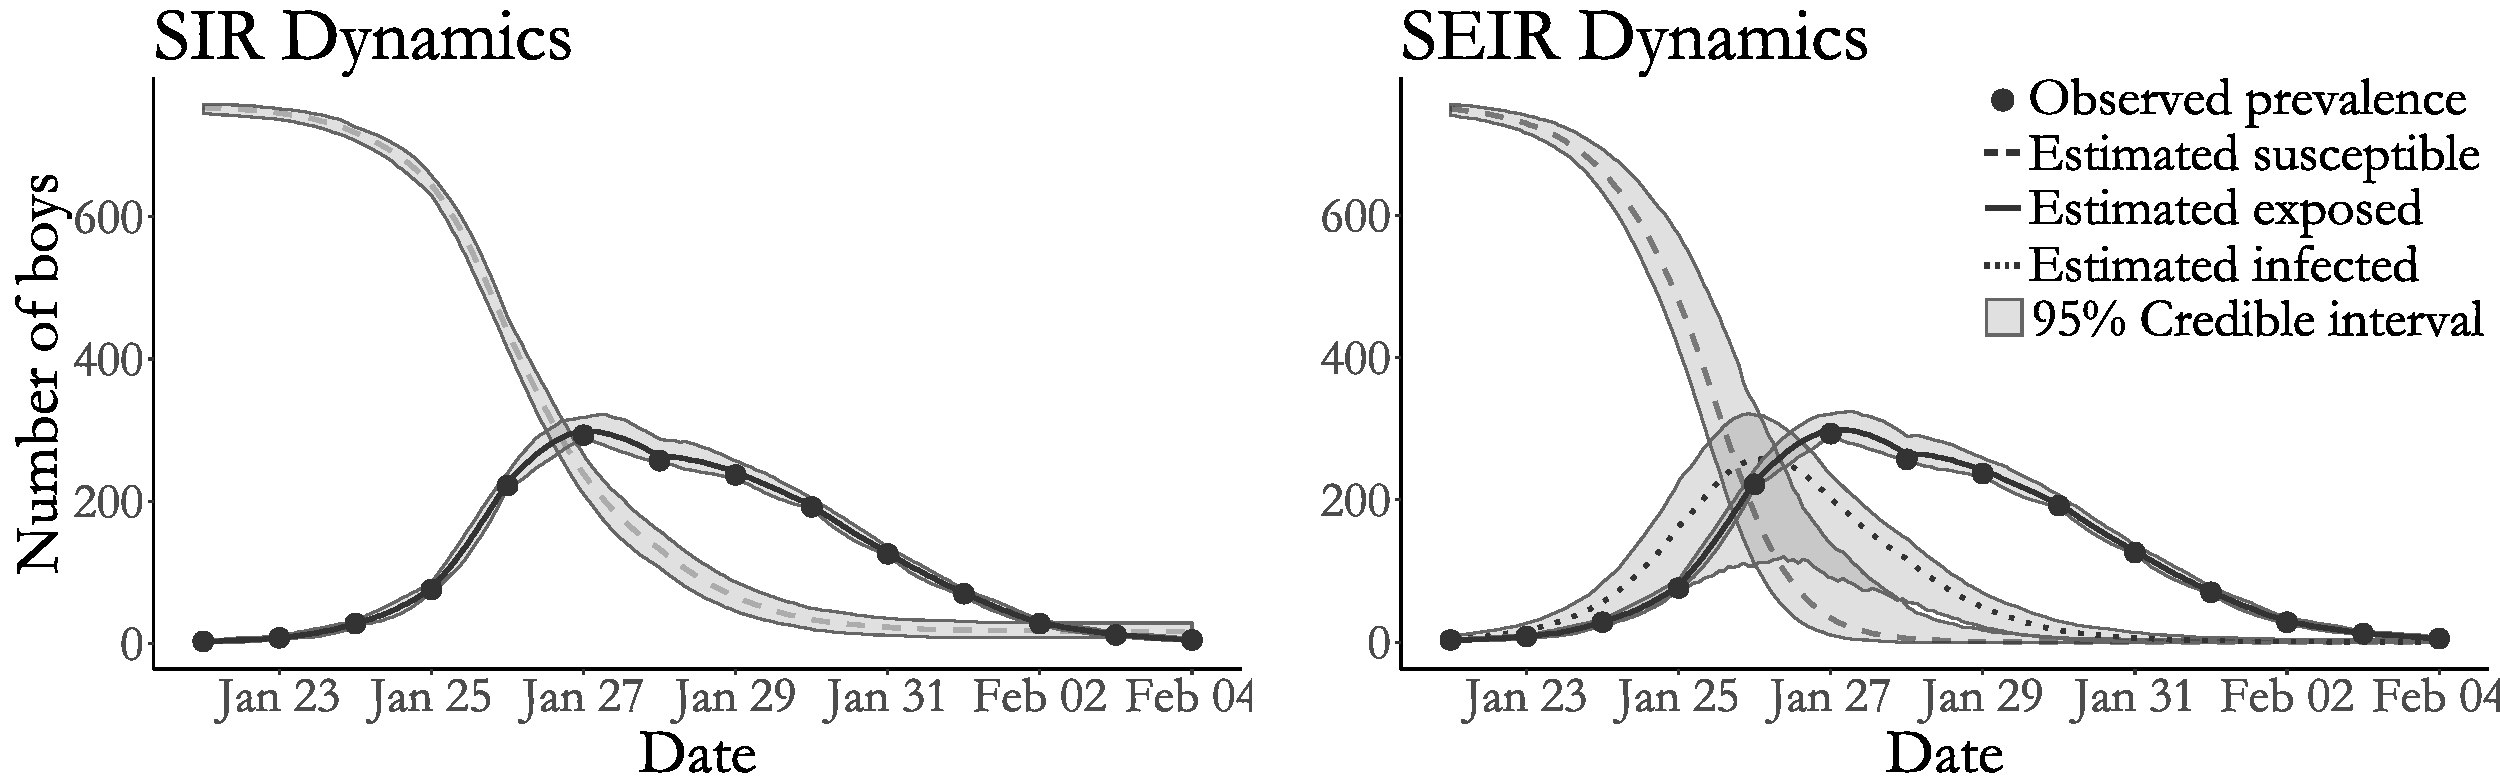
\includegraphics[width=\linewidth]{figures/bbs_latent_posts.pdf}
	\caption[Boarding school data and latent posterior under SIR and SEIR dynamics.]{Boarding school data, pointwise posterior median estimates and pointwise 95\% credible intervals (grey shaded areas) under SIR and SEIR dynamics of the numbers of susceptible boys (dashed line), exposed boys (dotted line), and infected boys (solid line). Posterior estimates based on a thinned sample, with every 250$ ^{th} $ configuration retained.}
	\label{fig:bbs_dat}
\end{figure}

Together, the SIR and SEIR models suggest that cases were detected with high probability and that the outbreak, though aggressive, was not atypical given the closed environment in which it occurred. The posterior median estimates of the detection probability, roughly 0.98 for both models (SIR 95\% BCI: 0.92, 1.00; SEIR 95\% BCI: 0.91, 1.00), suggested that while almost all of the infectious boys were detected, a handful of cases went unnoticed. The posterior median recovery rate under SIR dynamics corresponds to an average period of 2.16 days (95\% BCI: 1.99, 2.37) during which an infectious boy could transmit an infection to other boys before being confined to the infirmary. Under SEIR dynamics, the posterior median average infectious period was 2.12 days (95\% BCI: 1.95, 2.33), and the posterior median average latent period was 1.19 days (95\% BCI: 0.84, 1.51). These results are consistent with the typical progression of influenza, in which individuals typically incubate for between one to four days before symptoms manifest, and are typically infectious for one day before, and up to a week after, symptom onset \citep{cdcFlu}. The posterior median estimates of $ R_0 $ were 3.89 (95\% BCI: 3.40, 4.47) under SIR dynamics, and 10.38 (95\% BCI: 7.40, 14.11) under SEIR dynamics. Previous analyses of this dataset with trajectory matching estimate $ R_0 $ to be roughly 3.7 for the SIR model and 35.9 for the SEIR model \citep{wearing2005, keeling2008}, though we note that these estimates are based on deterministic models that do not properly account for distributional properties of the data. Our results for both models are also in agreement with estimates of SIR and SEIR model dynamics under a negative binomial emission distribution (see Section \ref{sec:bbs_neg_binom}).

\begin{figure}
	\centering
	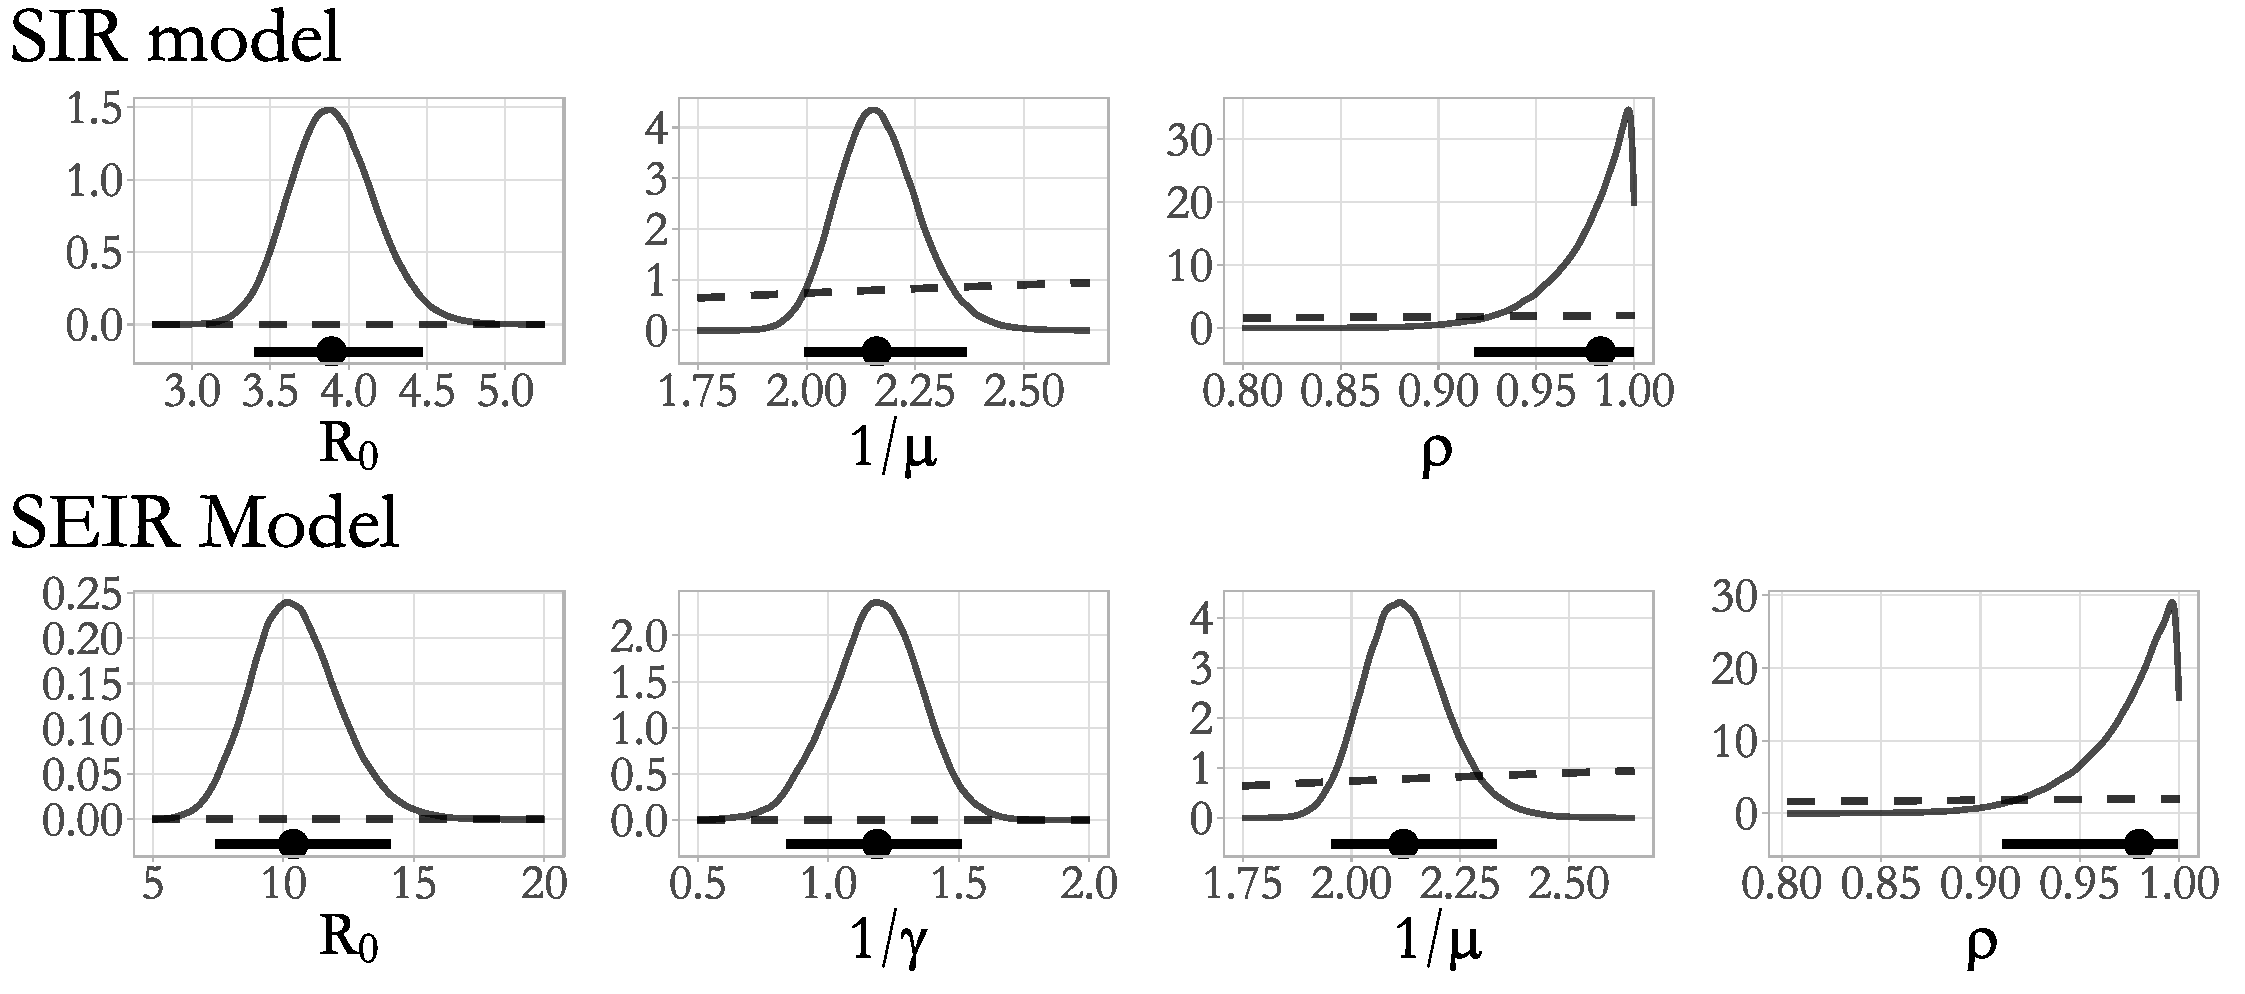
\includegraphics[width=0.95\linewidth]{figures/bbs_densities.pdf}
	\caption[Posterior estimates of SIR and SEIR model parameters fit to British boarding school outbreak data.]{Posterior density estimates for $ R_0 = \beta N /\mu $, the mean latent and infectious periods, $ 1/\gamma $ and $ 1/\mu $, and the binomial sampling probability, $ \rho $, from SIR and SEIR model parameters fit to the British boarding school data (solid lines). The posterior median and 95\% Bayesian credible intervals are drawn below the density plots (solid lines with circles). The implied prior densities (dashed lines) for $ R_0 $ and the latent and infectious periods, and the prior density for the binomial sampling probability, are plotted over the posterior ranges.}
	\label{fig:bbs_densities}
\end{figure}

\section{Discussion}
\label{sec:bda_discussion}

We have presented an agent--based Bayesian DA algorithm for fitting SEMs to disease prevalence time series counts. This was previously difficult, if not computationally infeasible, to carry out using traditional agent--based DA methods in the absence of subject--level data. Although we outlined the algorithm in the context of fitting an SIR model to binomially distributed prevalence data, our algorithm represents a general solution for fitting SEMs to prevalence counts. In simulations and the applied example, we fit SEIR and SIRS models to prevalence data, and in the supplement also fit SIR and SEIR models with a negative binomial emission distribution to the British boarding school data. We have demonstrated that our algorithm yields approximately valid inference when the population size is misspecified. Moreover, our algorithm is usable in settings where simulation--based methods, such as PMMH, break down due to misspecification of the SEM. Finally, our DA algorithm is carried out entirely at the subject level, making it possible to also incorporate subject--level covariates and household structure, or to fit models to subject--level data. 

There are two fundamental limitations of agent-based DA methods from which our algorithm is not excepted. First, the bookkeeping required to track the collection of subject--paths increases in size and complexity as the number of events grows large. Attempts to fit stochastic epidemic models in large populations using agent-based DA may be thwarted by prohibitive computational overhead. MCMC run times using our implementation, which was coded for reliability rather than speed, substantially degraded once the assumed population size was greater than a few thousand people. Second, we suspect that MCMC mixing in large populations could eventually become too slow for agent--based DA to be of practical use, even if solutions could be found for the computational bottlenecks. As the population size gets large, perturbations to the likelihood from re-sampling one subject at a time become relatively less significant. For this reason, we view extensions for jointly sampling multiple subject--paths as a critical step in mitigating slow MCMC mixing in large populations.

To conclude, we would like to comment on directions for future work that could be pursued. The DA algorithm in this paper addresses the problem of fitting SEMs to prevalence data. This type of data summarizes total number of infections in the population at a particular time. However, outbreak data often consist of incidence counts, which are the number of new cases accumulated in each inter-observation interval. Extending our DA algorithm to accommodate incidence data is an important next step and should be straightforward in situations where the state space for the subject level process is finite --- for instance, if a subject cannot become reinfected more than once or twice in a given inter-observation interval. Another line of inquiry involves improving the computational efficiency of the algorithm. One possibility would be to use a coarse grid for the time--varying force of infection used in each subject--path proposal, and to approximate the transition probabilities in the HMM step of the algorithm. For example, we could propose each subject--path conditionally on the disease states of all other subjects but assume that the force of infection is each inter--observation interval is fixed. This might lead to more subject--paths being rejected, but the loss could well be offset by not having to as many matrix exponentials. Finally, we note that the algorithm could also be used to fit semi--Markov models where transition probabilities depend on the duration of state occupancy. This would require a modification of the complete data likelihood and the Metropolis--Hastings ratio, though we could retain the Markovian structure of the proposal and possibly avoid costly rejected proposals by using a phase--type distribution to approximate the target semi--Markov process.